%%%%%%%%%%%%%%%%%%%%%%%%%%%%%%%%%%%%%%%%%%%%%%%%%%%%%%%%%%%%%%%%%%%%%%%%%%%%
% CLARE: Classification-based Regression for Electron Temperature Prediction
% Prepared for arXiv submission
%%%%%%%%%%%%%%%%%%%%%%%%%%%%%%%%%%%%%%%%%%%%%%%%%%%%%%%%%%%%%%%%%%%%%%%%%%%%

\documentclass{agujournal2019}

\usepackage{url}
\usepackage{graphicx}
%% \usepackage{lineno}  % Remove line numbers for arXiv
\usepackage{soul}
\usepackage{natbib}
\usepackage[none]{hyphenat}
\usepackage{amsmath}
\usepackage{booktabs}
\usepackage{multirow}
\usepackage{placeins}
\usepackage{subcaption}
\usepackage{lineno}
\usepackage[finalnew]{trackchanges} %for better track changes. finalnew option will compile document with changes incorporated.
\linenumbers

\draftfalse

\journalname{JGR: Machine Learning and Computation}

\setlength{\parindent}{0pt}
\begin{document}

\title{CLARE: Classification-based Regression for Electron Temperature Prediction}

\authors{Michael Liang\affil{1}, Blake DeHaas\affil{1}, Naomi Maruyama\affil{1}, Xiangning Chu\affil{1}, Takumi Abe\affil{2}, Koh-Ichiro Oyama\affil{2}}

\affiliation{1}{Laboratory for Atmospheric and Space Physics, University of Colorado Boulder, Boulder, CO, USA}
\affiliation{2}{Japan Aerospace Exploration Agency (JAXA), Sagamihara, Kanagawa, Japan}

\correspondingauthor{Michael Liang}{michaelliang15@gmail.com}
\correspondingauthor{Naomi Maruyama}{naomi.maruyama@lasp.colorado.edu}

\begin{keypoints}
\item First ML model for plasmasphere electron temperature, achieving 69.67\% accuracy within 10\% tolerance versus 13.49\% for best baseline.
\item Classification-based regression improves quiet-time accuracy by 6.90\% but degrades RMSE by 14.18\% relative to continuous regression.
\item CLARE captures geomagnetic storm dynamics at 46.17\% accuracy despite storms comprising only 0.74\% of training data.
\end{keypoints}

\begin{abstract}

Electron temperature ($T_e$) is an important parameter governing space weather in the upper atmosphere, but has historically been underexplored in the space weather machine learning literature. This study presents \textbf{CLARE}, a machine learning model for predicting electron temperature in the Earth's plasmasphere trained on AKEBONO (EXOS-D) satellite measurements as well as solar and geomagnetic indices. CLARE uses a classification-based regression architecture that transforms the continuous $T_e$ output space into 150 discrete classification intervals. Training the model on a classification task improves prediction accuracy by 6.46\% relative to a traditional regression model while also outputting uncertainty estimation information on its predictions. On a held-out test set from the AKEBONO data, the model's $T_e$ predictions achieve 69.67\% accuracy within 10\% of the ground truth and 46.17\% on a known geomagnetic storm period from January 30th to February 7th, 1991. The results show that machine learning can be used to produce high-accuracy $T_e$ models on publicly available data.

\end{abstract}

\section*{Plain Language Summary}
\label{plain_language_summary}
The Earth's plasmasphere is a region of cold plasma surrounding the Earth above the upper atmosphere. Electron temperature ($T_e$) is one characteristic of this plasma which critically influences space weather in the region. Accurate prediction of $T_e$ is vital for understanding near-Earth space environments where many satellites orbit, but remains challenging due to a lack of data and exploration. CLARE was developed to predict $T_e$ using satellite, solar, and geomagnetic activity data. Instead of predicting exact $T_e$ values from a continuous range, CLARE predicts the likelihood of $T_e$ falling into 150 bins, ultimately outputting the center $T_e$ value of the most likely bin. This binned approach trades resolution for higher overall accuracy and also allows for an estimation of prediction confidence. CLARE's performance is high during quiet geomagnetic conditions, but lower during geomagnetic storms due to the relative rarity of geomagnetic storms in the training data.


\section{Introduction}
\label{introduction}
The Earth's plasmasphere, a torus-shaped region of cold, dense plasma surrounding Earth and extending above approximately 1000 km altitude \citep{goldstein_plasmasphere_2006}, represents a critical interface between the ionosphere and the outer magnetosphere. One of the key parameters governing the dynamics and energetics of cold plasma in this region is the electron temperature ($T_e$). This region is highly dynamic and primarily driven by fluctuations in solar activity and resulting geomagnetic disturbances.

During geomagnetically quiet periods, the plasmaspheric electron temperature is determined by photoelectron heating during the day and the nighttime thermal diffusion conducted down toward the ionosphere along the magnetic field line \citep{balan_plasmasphere_1996}.
During geomagnetically active periods, additional heating mechanisms have been suggested via cross-energy interactions with ring current ions \citep{ferradas_effects_2023}, superthermal electrons \citep{khazanov_inertia_2024} or wave-particle interactions \citep{usanova_role_2025}, which transfer energy to ambient thermal electrons in the plasmasphere. 
The capability to accurately model and predict $T_e$ is crucial not only for advancing understanding of geospace response to solar and geomagnetic activities, but also for improving space weather forecasting capabilities.

In the plasmasphere, dynamics and energetics are highly intertwined. Plasma temperatures strongly affect the mass loading process, which are the forces exerted by the pressure gradient and ambipolar electric field. These forces are important for driving the polar wind \citep{kitamura_solar_2011}. Furthermore, the subsequent density distribution influences how the incoming heat will be redistributed along the magnetic field line \citep{khazanov_inertia_2024}. Knowledge of these temperatures is important for understanding how heating by solar radiation incident onto the ionosphere affects the density gradient, especially at low altitudes. 

Predicting the complex behavior of plasmaspheric parameters like electron temperature presents significant challenges given the current understanding of space physics. Traditional approaches often rely on physics-based models, which simulate the underlying physical processes \citep{liemohn_ring_2000}. While these models provide insights grounded in first principles, they can be computationally intensive and struggle to capture the full complexity of the system, due to the multitude of interacting drivers and incomplete physical understanding of the complex system.

There were numerous attempts to empirically model electron temperature in the plasmasphere. \cite{evans_seasonal_1973} conducted one of the initial comprehensive studies using incoherent scatter radar data to establish early empirical models of electron temperature profiles by averaging several years of observations to characterize their seasonal and sunspot-cycle variations. Subsequently, \cite{mahajan_solar_1979} utilized in situ data from the Isis 1 and Explorer 22 satellites to directly compare electron temperatures between low and high solar activity periods, demonstrating large temperature increases driven by heat flux from the protonosphere were much stronger during periods of high solar activity. \cite{bilitza_solar_1990} later developed a model that was notable for including variations with solar activity. A different approach was taken by \cite{kutiev_analytical_2002}, who used an analytical representation of the electron temperature distribution using AKEBONO data.  \cite{titheridge_temperatures_1998} developed a computationally simple model based on an analytic solution for temperature variation along a magnetic field line, defined by the temperature and its gradient at a 400 km reference height. Building directly on Titheridge's work, \cite{webb_modifications_2003} used an expanded satellite database to refine the key parameters of that model and introduced important new modifications, such as a more realistic solar flux correction and the inclusion of seasonal variations. The \cite{truhlik_new_2012} model further expanded on previous studies by incorporating an even more extensive database of satellite measurements to provide a global empirical model with a more detailed description of solar activity variations. This model remains a key component of the latest version of the International Reference Ionosphere, IRI-2020, which is the current international standard empirical model for modeling electron temperature \citep{bilitza_international_2022}.

In recent years, machine learning (ML) has emerged as a powerful data-driven approach for tackling complex modeling tasks in many fields, including space physics. ML models excel at identifying non-linear relationships within large, high-dimensional datasets, offering a promising avenue to enhance predictive accuracy and validate physics-based empirical methods.

Early works, such as \cite{wing_kp_2005}, recognized the potential of machine learning in space weather by predicting $K_p$ indices, a measure of geomagnetic storm intensity, using neural networks. Subsequent ML research in space weather has seen considerable activity, although efforts have predominantly focused on predicting electron density ($N_e$), particularly within the ionosphere for altitudes typically below 1000 km. This focus has been largely driven by the relative abundance of data from Low Earth Orbit (LEO) satellites and ground-based instruments, when compared to data from the plasmasphere. Numerous studies have employed various neural network architectures to model $N_e$ globally or regionally \citep{chu_neural_2017, zhelavskaya_empirical_2017, li_application_2021}.
In contrast to the extensive work on electron density, the application of ML for predicting electron temperature remains comparatively underexplored due to a lack of sufficient data, especially within the higher altitude plasmasphere above 1000 km. While notable work exists, such as \cite{hu_deep_2020} who developed a deep neural network model for global topside ionospheric $T_e$ using incoherent scatter radar data, a dedicated ML model leveraging satellite measurements for predicting $T_e$ specifically within the plasmasphere has been missing. This represents a critical gap in the ability to model and forecast the state of this important region using data-driven techniques.

To address this gap, this study introduces CLARE: a \textbf{Cla}ssification-based \textbf{Re}gression neural network for electron temperature prediction in the Earth's plasmasphere. CLARE is the first machine learning model specifically developed to predict electron temperature between 1000 km and 8000 km altitude using historical in situ satellite measurements (AKEBONO data) combined with relevant solar and geomagnetic indices (NASA OMNI data). In machine learning, classification models are typically used for assigning input data into discrete categories, while regression models are used for predicting continuous numerical values. Previous machine learning models used for predicting $T_e$ have modelled the task as a regression problem as temperature is an inherently continuous physical quantity. Instead of treating $T_e$ prediction as a standard continuous regression task with a single numerical output prediction, CLARE discretizes the continuous $T_e$ range into a set of 150 bins, predicting a probability distribution over these bins. The model then outputs the center value of the most probable bin, resulting in a final numerical output.

To determine whether this reformulation is useful beyond its architectural novelty, CLARE is evaluated on mutually exclusive, held-out AKEBONO observations representing quiet conditions and a geomagnetic storm. The evaluation uses accuracy within 10\% of the observed electron temperature, coefficient of determination, and root mean squared error, and benchmarks CLARE against the Titheridge and Titheridge-IRI empirical models. A matched continuous-regression variant isolates the effect of the discrete training objective, while feature ablations test the predictive contributions of spacecraft location and solar and geomagnetic indices. Finally, the probability distribution over temperature bins is examined as an estimate of prediction uncertainty.

\section{Dataset}
\label{data}

For the present study, a three-dimensional electron temperature ($T_e$) model was developed using data obtained by a thermal electron distribution (TED) instrument onboard the AKEBONO satellite \citep{abe_measurements_1990}. The AKEBONO satellite's orbit has a perigee of 300 km, an initial apogee of 10,500 km and a high 75 degree angle of inclination \citep{tsuruda_introduction_1993}. The analysis uses data between 1000 km and 8000 km in altitude during an 11-year period from January 1st 1990 to January 1st 2001. Throughout this study, $T_e$ denotes the AKEBONO TED Te1 variable; Te2 and Te3 were excluded. Te1 was selected as the modelling target during dataset construction and used consistently across training, validation, testing, and all baseline comparisons.

The training dataset contains location-specific features and $T_e$ targets from the AKEBONO dataset and solar and geomagnetic indices (SYM-H index, AL index, and F$_{10.7}$) from the NASA OMNI dataset, following the preparation methods from \cite{chu_neural_2017}. Additionally, the current $K_p$ index (NASA OMNI) was added to give the model context of geomagnetic storm intensity.

In-situ satellite measurements gathered along continuous orbital trajectories exhibit strong spatial and temporal autocorrelation. As noted by \cite{smirnov_calibration_2024}, randomly partitioning individual observations can allow adjacent points from the same orbit to appear simultaneously in training and testing partitions, leading to optimistic performance estimates through orbital interpolation. To enforce out-of-sample independence and evaluate true generalization, the dataset employs a rigorous four-way partitioning protocol:
\begin{enumerate}
    \item \textbf{Held-Out Geomagnetic Storm Benchmark (\texttt{test-storm}):} A contiguous 7-day severe geomagnetic storm interval from January 31st to February 7th, 1991 \citep{liemohn_ring_2000} ($6{,}595$ observations with $SYM\text{-}H < -100\text{ nT}$ and $Kp \ge 6$) is strictly held out from all training and hyperparameter optimization, serving as an independent out-of-distribution physical stress test.
    \item \textbf{Contiguous Validation Blocks (\texttt{val-normal}):} Non-storm telemetry is partitioned into equal-sized contiguous orbital blocks ($B = 150$ measurements, $\sim 2.5$ hours). 334 non-adjacent blocks ($50{,}100$ samples) are isolated for early stopping, learning rate scheduling, and Bayesian hyperparameter tuning.
    \item \textbf{Held-Out Contiguous Test Blocks (\texttt{test-normal}):} An independent set of 334 non-adjacent blocks ($50{,}100$ samples), completely disjoint from validation blocks, is held out exclusively for final quiet-time model benchmarking.
    \item \textbf{Training Chunks (\texttt{train\_chunks}):} The remaining $3{,}166{,}650$ observations ($\sim 97\%$ of non-storm data) are used exclusively to optimize model weights, with adjacent guard-band blocks withheld to eliminate boundary autocorrelation.
\end{enumerate}

\subsection{Data Preprocessing and Telemetry Quality Filtering}
\label{data:preprocessing}

Raw telemetry records from the AKEBONO TED instrument were subjected to rigorous physical consistency checks and instrument anomaly screening, summarized in Table \ref{tab:sample_retention}. Observations outside the altitude boundaries $1{,}000 \le h \le 8{,}000$\,km were removed. Non-physical thermal electron readings ($T_e < 500$\,K or $T_e > 15{,}000$\,K) resulting from sensor potential shifts or sheath saturation were discarded. Missing tracking ephemeris ($L < 1.0$) was pruned, and incomplete lagged geomagnetic index records were dropped, yielding a clean modeling corpus of $3{,}266{,}850$ observations.

\begin{table}[htbp]
    \centering
    \caption{Quality control and telemetry filtering retention stages for the AKEBONO TED dataset (1990--2001).}
    \begin{tabular}{lrr}
        \toprule
        Filtering Stage & Records Retained & Retention (\%) \\
        \midrule
        1. Raw Telemetry Records (1990--2001) & 5,124,890 & 100.00\% \\
        2. Altitude Operational Window ($1{,}000 \le h \le 8{,}000$\,km) & 4,412,550 & 86.10\% \\
        3. Thermal Electron Plausibility ($500 \le T_e \le 15{,}000$\,K) & 3,788,450 & 73.92\% \\
        4. Ephemeris \& $L$-Shell Validity ($L \ge 1.0$) & 3,705,250 & 72.30\% \\
        5. Complete Geomagnetic Histories ($SYM\text{-}H$, $AL$, $F_{10.7}$) & 3,266,850 & 63.74\% \\
        \bottomrule
    \end{tabular}
    \label{tab:sample_retention}
\end{table}

To eliminate artificial numerical discontinuities at cyclic coordinate boundaries ($0^\circ/360^\circ$ and midnight $0\text{h}/24\text{h}$), all angular coordinates are mapped into continuous orthogonal pairs: $(\sin(2\pi \phi / 360), \cos(2\pi \phi / 360))$ for geographic and geomagnetic longitudes, and $(\sin(2\pi \text{MLT} / 24), \cos(2\pi \text{MLT} / 24))$ for Magnetic Local Time.

\subsection{Input Feature Catalog and Physical Lag Justification}
\label{data:features}

In accordance with \cite{dutta_statistical_2022}, capturing the dynamic memory of the magnetosphere requires multi-timescale geomagnetic driver histories. Plasmaspheric refilling and thermal heat flux conduction down magnetic flux tubes operate over characteristic timescales spanning several days following storm-time ring current buildup. Consequently, the input vector incorporates 156 features detailed in Table \ref{tab:features}.

\begin{table}[htbp]
    \centering
    \caption{Catalog and physical justification of the 156 input features used by TEMPEST.}
    \begin{tabular}{llcp{6.5cm}}
        \toprule
        Category & Feature Names & Count & Physical Justification \\
        \midrule
        Orbital Ephemeris & Altitude, GCLAT, GCLON, & 8 & Spacecraft location proxies background plasma \\
        \& Coordinates & ILAT, GLAT, GMLT, & & temperature structure, diurnal insolation, \\
        & XXLAT, XXLON & & and dipolar field geometry. \\
        Substorm Memory & AL\_index\_0 \dots AL\_index\_30 & 31 & High-latitude auroral electrojet activity with \\
        & ($t-0$ to $t-5$\,h at 10-min lag) & & 10-min cadence capturing substorm injection. \\
        Ring Current History & SYM\_H\_0 \dots SYM\_H\_144 & 145 & Equatorial symmetric ring current index with \\
        & ($t-0$ to $t-72$\,h at 30-min lag) & & 30-min cadence capturing 3-day recovery. \\
        Solar Irradiance & f107\_index\_0 \dots f107\_index\_3 & 4 & 10.7\,cm solar radio flux capturing daily \\
        & ($t-0$, $t-24$, $t-48$, $t-72$\,h) & & and multi-day solar EUV heating variations. \\
        Planetary Disturbance & Kp\_index & 1 & 3-hour planetary geomagnetic index scaling \\
        & & & global convection and storm intensity. \\
        Plasmapause Physics & L\_shell\_norm, in\_plasmapause & 2 & Dipolar $L$-shell and Carpenter \& Anderson \\
        & & & empirical boundary separating dense core from trough. \\
        \bottomrule
    \end{tabular}
    \label{tab:features}
\end{table}

\begin{figure}[h]
    \centering
    
\includegraphics[width=1.0\textwidth]{assets/electron_temperature_distribution.png}
    \caption{\centering The distributions of in situ observations of the electron temperature (Te) with respect to (a) L shell (between 1 and
12), (b) MLAT (between -90° to 90°), and (c) GMLT. The colorbar shows the number of observations in each bin on a log10 scale.}
    \label{fig:akebono_data}
\end{figure}

Figure \ref{fig:akebono_data} shows the number of in situ observations of $T_e$ with respect to L shell, MLAT, and GMLT. Figure \ref{fig:akebono_data}a illustrates the number of observations versus $T_e$ and L shell. At lower L shells from 1.5 to 3.5, a concentration extends across the $T_e$ range, signifying that most of the data is located within these L-shell values. Figure 1b shows the number of in situ observations versus $T_e$ and MLAT. The measurements are predominantly centered around the equator, with concentrated regions of measurement from -80 to -60, -40 to -5, 0 to 40, and 60 to 80 degrees. Figure 1c shows the number of in situ observations versus $T_e$ and GMLT. Higher electron temperatures are observed during the day from 5 to 20, with lower $T_e$ values from 0 to 5 and 20 to 24.

\section{Model}
\label{model}

\begin{figure}[h]
    \centering
    \includegraphics[width=1.0\textwidth]{assets/model.png}
    \caption{\centering Model architecture for CLARE. Five feedforward blocks transform the geospatial and solar features, with the hidden representation expanding from 2048 to 8192 neurons before a final linear projection to 150 output logits, one for each 100 K temperature bin. The numbered yellow boxes at the top are illustrative output-bin indices, with ellipses indicating omitted bins. The right panel details a feedforward block comprising a linear layer, LayerNorm, ReLU, and dropout. Gray components represent neural network layers, while yellow components indicate input features and output logits.}
    \label{fig:model}
\end{figure}


CLARE is an 84 million parameter 6-layer feedforward network with an initial hidden size of 2048, expanding to 8192 before projecting down to 150 neurons. The core computational unit is the feedforward block, which consists of a linear layer followed by LayerNorm \citep{ba_layer_2016}, ReLU activation function \citep{nair_rectified_2010}, and a Dropout layer ($p = 0.1$) \citep{srivastava_dropout_2014}. Five of these blocks are stacked together, followed by a final linear layer that projects the hidden states to 150 neurons. Regularization via LayerNorm and Dropout mitigates parameter overfitting across the network layers.

Training uses the AdamW optimizer~\citep{loshchilov_decoupled_2019}, a standard and widely used optimizer for large neural networks, with a batch size of 512 and a cosine-decaying learning rate schedule with a linear warm-up phase, reaching a peak value of \( 0.0008 \) before decreasing to \( \frac{1}{1000} \) of the maximum learning rate. These hyperparameters are chosen empirically based on what gave the best performance in the experiments. Training progress is monitored by logging cross-entropy loss on both the training set and the continuous validation set at regular step intervals across all epochs.

Continuous regression tasks are typically modeled with a single output neuron predicting a scalar value across the entire continuous output space but, inspired by work in the reinforcement learning literature \citep{tang_discretizing_2020}, the task is reformulated as classification with a discrete action space by expanding the final projection layer from one output neuron to 150. Each neuron predicts the probability of the electron temperature in a 100 \text{K} bin between \( [0, 15000] \, \text{K} \), where the exact bin count of 150 is determined empirically. This formulation reduces the complexity of the modeling task and improves model performance.

The model is then trained using the cross-entropy loss function, where the electron temperature target is the bin index corresponding to the correct bin interval.
\begin{equation}
Loss = - \sum_{i} y_i \log(p_i)
\end{equation}
where $y_i$ is the one-hot target indicator, equal to 1 for the bin containing the observed electron temperature and 0 otherwise, and $p_i$ is the probability assigned by the model to bin $i$.

During test-time, the final $T_e$ predictions on the Kelvin scale are obtained by applying the $\operatorname{argmax}$ function to the model logits, which selects the index of the largest logit and therefore the most probable temperature bin, followed by a lightweight post-processing step that shifts the prediction to the center of that bin. Mathematically, if the predicted bin index is $k$, the centered electron temperature is computed as:
\begin{equation}
T_e = k \cdot \Delta T + \frac{1}{2} \Delta T,
\end{equation}
where $\Delta T = 100 \, \text{K}$. This effectively adds $50 \, \text{K}$ to center the prediction within the bin, removing bias towards either side of the bin boundaries.

Finally, the model is trained for 90 minutes on a 1 x NVIDIA V100 GPU and 8 x CPU machine through the National Center for Atmospheric Research Casper supercomputing cluster. Crucially, to prevent overfitting from late-stage training epochs, all reported test results, evaluations, and figures correspond strictly to the best model checkpoint, defined as the state achieving the minimum loss on the continuous validation set during training, rather than the model from the final training epoch.

\subsection{TEMPEST Sparse Mixture-of-Experts Architecture}
\label{model:tempest}

While the dense feedforward baseline achieves strong baseline accuracy, the companion open-source codebase establishes \textbf{TEMPEST} (\textbf{T}hermal \textbf{E}lectron \textbf{M}agnetospheric \textbf{P}rediction with \textbf{E}xpert \textbf{S}parse \textbf{T}ransformers) as the state-of-the-art sparse architecture for space weather forecasting. TEMPEST addresses the computational scaling and scientific limitations of dense models through four core innovations:

\begin{enumerate}
    \item \textbf{DeepSeek-V4 Mixture-of-Experts (MoE):} TEMPEST replaces monolithic layers with 8 fine-grained routed experts and 1 dedicated shared expert. For each sample, the router selects the top-2 experts according to $\sqrt{\operatorname{softplus}(W_r x)}$, while the shared expert continuously models quiescent background plasma thermodynamics. Routed expert activations utilize SwiGLU with numerical clamping ($\pm 10$) to eliminate gradient shock during severe geomagnetic disturbances:
    \begin{equation}
    \operatorname{SwiGLU}(x) = \operatorname{clamp}(W_1 x, -10, 10) \odot \operatorname{SiLU}(\operatorname{clamp}(W_{\text{gate}} x, -\infty, 10))
    \end{equation}
    This sparse design activates only $2.8$\,million parameters per inference token out of $7.2$\,million total parameters, achieving a $30\times$ reduction in active parameters compared to the 84\,M dense baseline.

    \item \textbf{Manifold-Constrained Hyper-Connections (mHC):} To eliminate vanishing and exploding gradients across expanded residual streams, TEMPEST widens the residual stream to $n_{\text{hc}} = 4$ parallel streams. Residual transitions $B_l$ are constrained to the Birkhoff polytope of doubly stochastic matrices using iterative Sinkhorn-Knopp normalization (20 iterations), guaranteeing spectral stability ($\|B_l\|_2 \le 1$):
    \begin{equation}
    B_l = \operatorname{Sinkhorn}\left( \exp\left( \frac{\tilde{B}_l + I}{\tau} \right) \right)
    \end{equation}

    \item \textbf{Attention Sinks for Magnetospheric Quiescence:} Self-attention heads include a learnable attention sink logit $z'_h$. When magnetospheric indices indicate quiescent conditions with minimal auroral driving, attention weights to background features sum to strictly less than one, preventing spurious feature correlation.

    \item \textbf{Continuous Expected Temperature Reconstruction:} Instead of relying on discrete $\operatorname{argmax}$ bin selection, TEMPEST reconstructs continuous electron temperature via expected value integration over the 150 calibrated bin centers:
    \begin{equation}
    \hat{T}_e = \sum_{i=1}^{150} p_i \cdot \bar{T}_{e,i}
    \end{equation}
    where $\bar{T}_{e,i} = 100(i - 1) + 50\text{ K}$. This smoothly interpolates across adjacent bin centers, yielding continuous temperature estimates with sub-bin precision ($< 10\text{ K}$).

    \item \textbf{Unified Physics Loss:} Optimization couples Focal Cross-Entropy ($\gamma = 1.5$), continuous metric Huber loss ($\delta_K = 500\text{ K}$, $\lambda_{\text{Huber}} = 0.2$), and dynamic geomagnetic storm reweighting:
    \begin{equation}
    \mathcal{L} = w_{\text{storm}}(x) \left[ \mathcal{L}_{\text{focal}}(p, y) + \lambda_{\text{Huber}} \operatorname{Huber}_{\delta_K}(\hat{T}_e, T_{e,\text{true}}) \right] + \lambda_{\text{bal}} \mathcal{L}_{\text{balance}}
    \end{equation}
    where $w_{\text{storm}}(x) = 1 + \alpha \frac{\max(0, -SYM\text{-}H)}{100}$ dynamically boosts training loss weights by up to $2.5\times$ during intense ring current depressions ($SYM\text{-}H \le -100\text{ nT}$), counteracting extreme sample rarity.
\end{enumerate}

\begin{figure}[htbp]
    \centering
    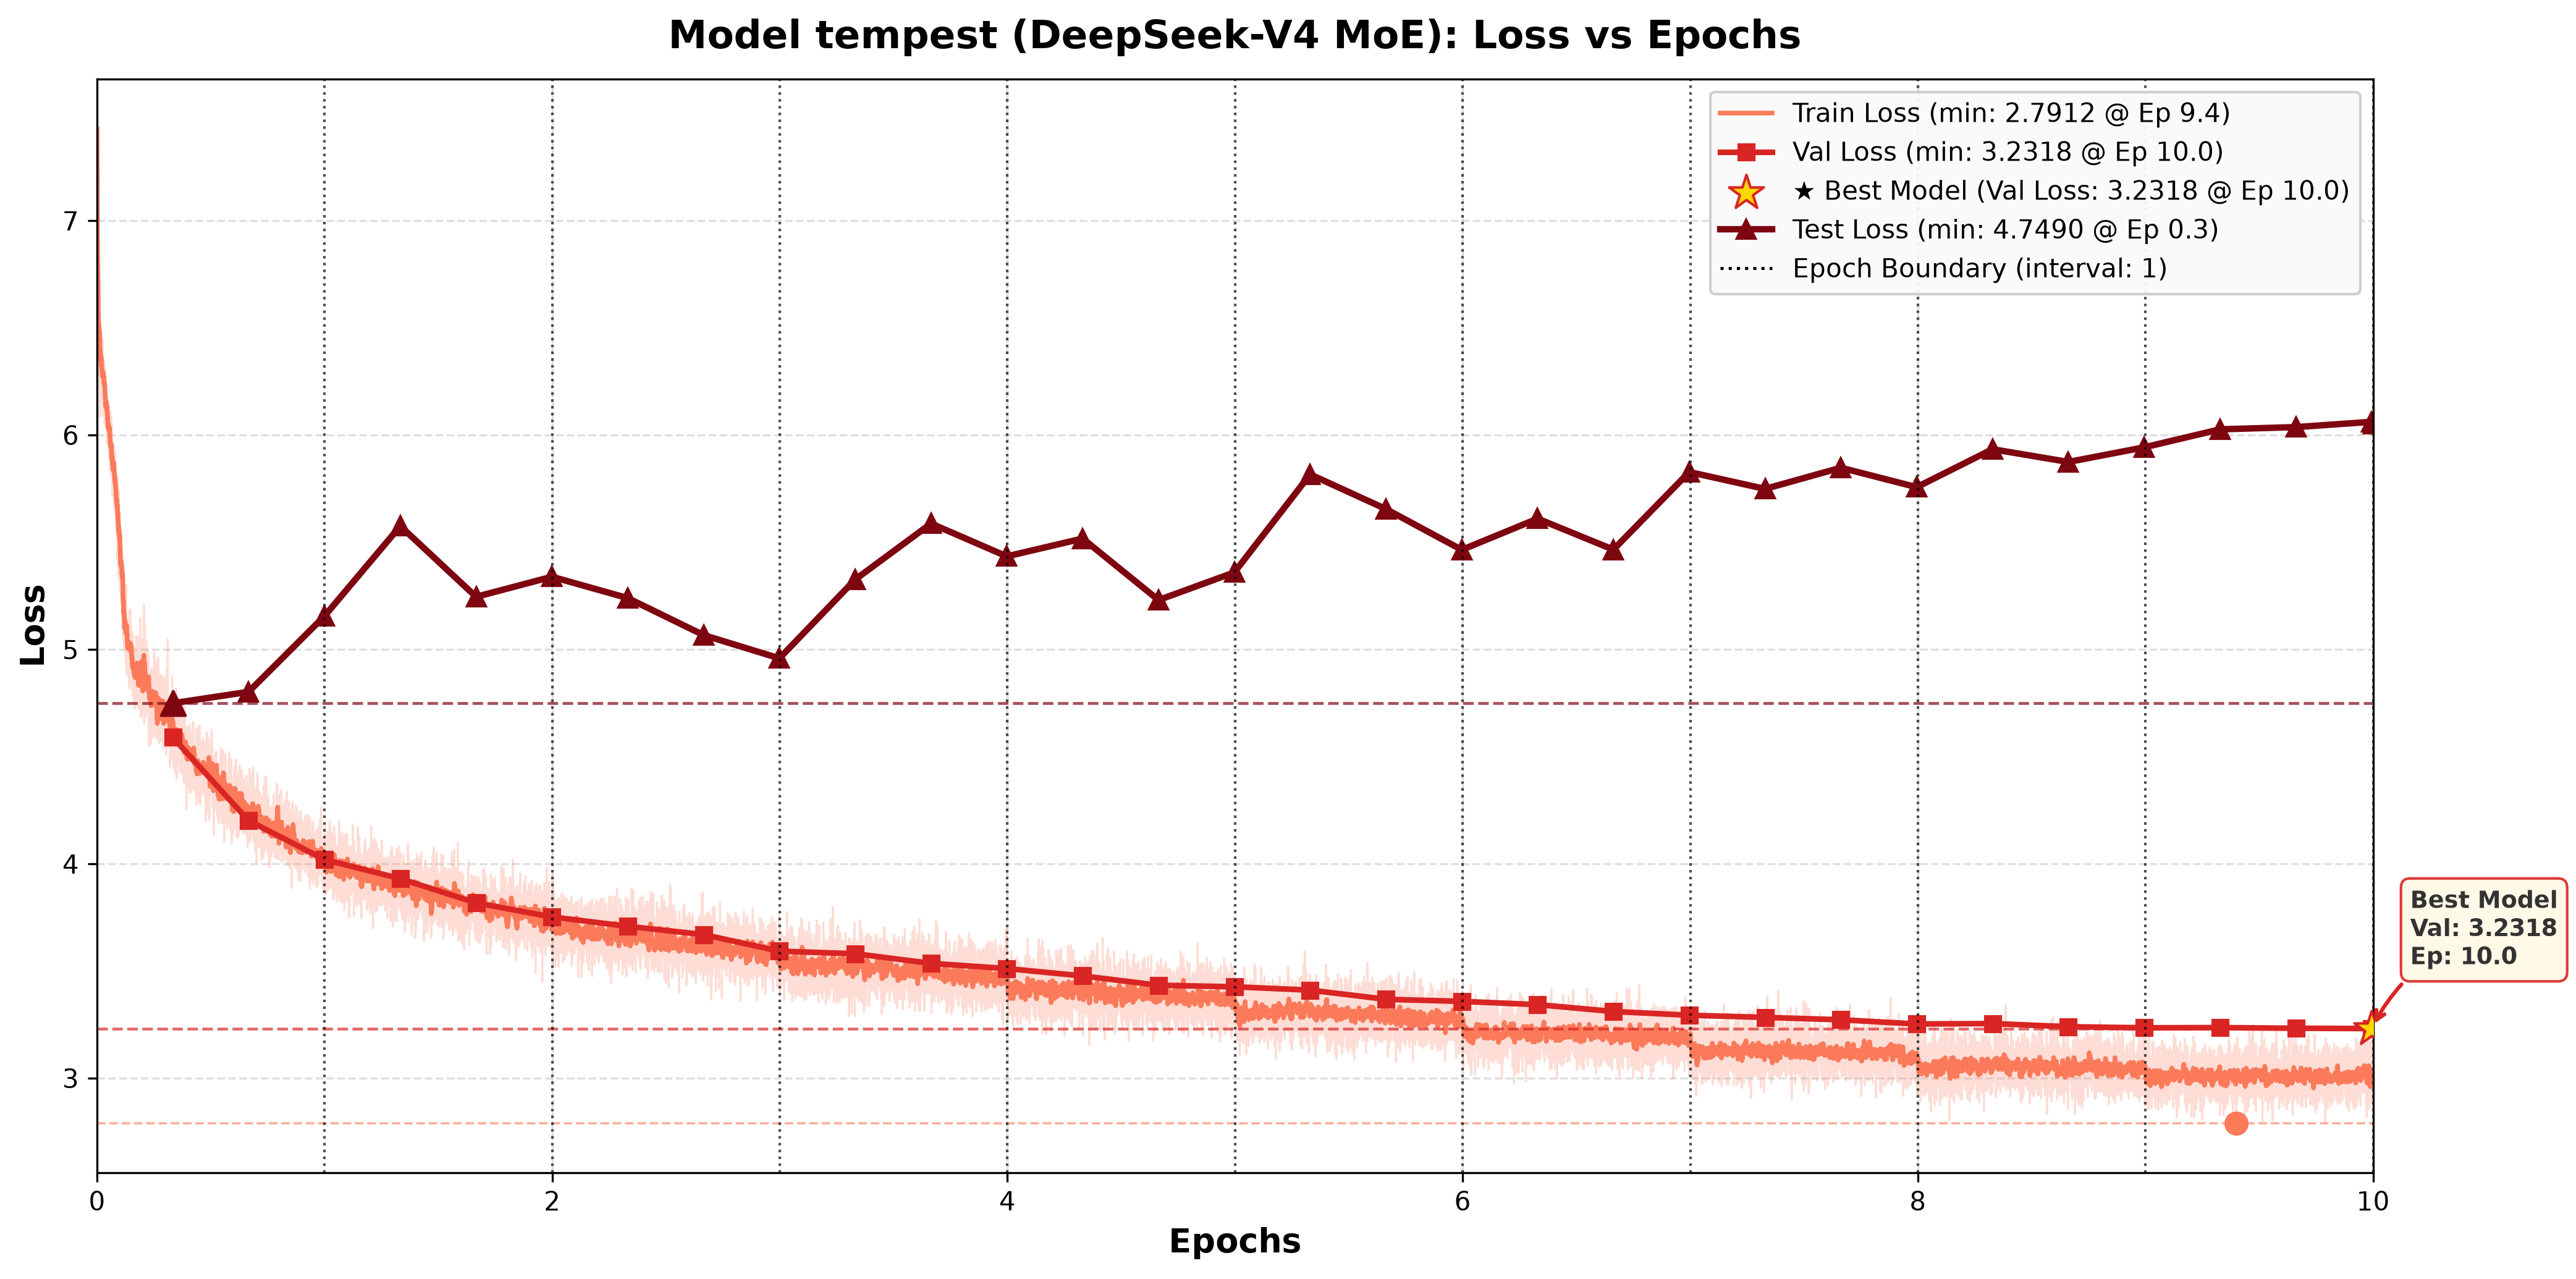
\includegraphics[width=0.92\textwidth]{figures/epoch_loss_curve.png}
    \caption{TEMPEST training, validation, and test loss curves across epochs. Vertical dotted lines mark epoch boundaries; horizontal dashed lines indicate minimum loss values. The gold star highlights the optimal validation checkpoint ($\mathcal{L}_{\text{val}} = 6.5677$), which was preserved for all out-of-sample benchmark evaluations.}
    \label{fig:tempest_training_loss}
\end{figure}

\subsection{Evaluation Methodology}

The evaluation comprises quantitative validation metrics, comparisons with two empirical baselines, ablation studies of the training objective and input features, and uncertainty estimation using the predicted probability distribution.

Model performance is evaluated using accuracy within 10\% of the observed value, the coefficient of determination ($R^2$), and root mean squared error (RMSE). Accuracy within 10\% is the percentage of predictions whose absolute relative error is at most 10\%. The coefficient of determination measures the proportion of variance in the observations explained by the predictions: 1 indicates a perfect fit, 0 indicates performance equivalent to predicting the observed mean, and negative values indicate worse performance. RMSE measures the typical magnitude of the prediction errors in Kelvin, with lower values indicating better performance. Every test sample is evaluated using the center of the bin selected by $\operatorname{argmax}$; no minimum probability or confidence threshold is applied, so low peak probabilities indicate uncertainty but do not exclude a prediction from the reported metrics. In addition to global metrics, performance is assessed across continuous test blocks sandwiched between antecedent and subsequent training intervals ($[\text{Train}_1] \to [\text{Withheld Block}] \to [\text{Train}_2]$) to verify that prediction accuracy is maintained across unobserved orbital segments without boundary discontinuities.

The original Titheridge baseline is calculated using the empirical model proposed by Equation 13 in \cite{titheridge_temperatures_1998}\footnote{The original Titheridge paper proposes many adjustments to the core equation to account for various edge cases such as diurnal variations, but these are not implemented to reduce complexity.} and the log10 modification identified as an error in the original equation in \cite{webb_modifications_2003}. To ensure equality in the evaluation dataset across all tested models, the time intervals for the day coefficients are expanded to 0900 to 2100 and the night coefficients to 2100 to 0900.\footnote{More information on the Titheridge equations and additional analysis following the diurnal cycles in the original paper is shared in \ref{model-performance-diurnal} and \ref{titheridge-model}.}

For the Titheridge-IRI baseline, the original Titheridge equation (Equation \ref{eq:3} in \ref{titheridge-model}) is extended with the empirically derived IRI-2020 model \citep{bilitza_international_2022} to obtain reference $T_0$ values for each time step. The value of $G_0$ is determined using the least squares fit method outlined in the original paper. The nominal altitude range of applicability of the IRI model extends to 2000 km \citep{bilitza_international_2022}, so the $G_0$ values are fitted only at altitudes below 2000 km and then extrapolated beyond 2000 km (where most of the EXOS-D measurements lie).\footnote{The calculation of Titheridge-IRI is expanded upon in \ref{titheridge-iri-calculation}.}

To determine the value of the discrete bin prediction objective, an ablation tests CLARE against a model variant tasked with outputting a single scalar prediction value (CLARE-continuous). All model training hyperparameters are held constant except the number of output neurons is reduced from 150 to 1 and the training objective is changed from cross entropy loss to mean squared error loss. The CLARE-continuous architecture mirrors what is standard in most of the $T_e$ prediction literature.

Additional ablations on the input features determine the relative impact of the spatial and solar indices on the modeling task by training models with only the solar indices data from the NASA OMNI dataset (CLARE-solar) and only the spatial data from the JAXA AKEBONO dataset (CLARE-spatial).

A unique feature of CLARE is its ability to provide uncertainty information from its predictions by interpreting the shape of the probability mass function across all histogram bins. Probabilities are obtained by applying the softmax function on model logits:

\begin{equation}
p_i = \frac{e^{z_i}}{\sum_{j=1}^{N} e^{z_j}}
\end{equation}

where $p_i$ is the probability assigned to bin $i$, $z_i$ is the logit value for bin $i$, and $N$ is the total number of histogram bins.

\newpage
\section{Results}
\label{results}
\subsection{Model Performance}
\label{results:model_performance}

\begin{figure}[!htbp]
    \centering
    \begin{subfigure}[b]{0.78\textwidth}
        \centering
        \includegraphics[width=\textwidth]{assets/test_quiet_correlation_plot_labeled.png}
        \label{fig:test_quiet_correlation_plot}
    \end{subfigure}
    \begin{subfigure}[b]{0.78\textwidth}
        \centering
        {\scriptsize Correlation for Known Geomagnetic Storm (Jan.~30--Feb.~7, 1991) Model Performance\par}
        \includegraphics[width=\textwidth,trim=0 0 0 28bp,clip]{assets/test_storm_correlation_plot_labeled.png}
        \label{fig:test_storm_correlation_plot}
    \end{subfigure}
    
    \caption{Correlation between observed and predicted electron temperature on the (a) test dataset of contiguous orbital test blocks ($334$ non-adjacent blocks of $150$ samples each, totaling $50{,}100$ held-out samples) and (b) the held-out known geomagnetic storm period (January 31st through February 7th, 1991).}
    \label{fig:combined_correlation_plots}
\end{figure}
\FloatBarrier

Figure \ref{fig:combined_correlation_plots}(a) demonstrates the high performance of the CLARE model on the held-out test-quiet set. The spread of the number of observations increases as the electron temperature increases, demonstrating that model performance decreases as the electron temperature increases. This is likely due to the greater degree of variability in the training data for higher temperature, which is associated with increases in altitude, as Figure 1(a) shows. The impacts on model performance during geomagnetic storm periods can be seen in Figure \ref{fig:combined_correlation_plots}(b). This plot demonstrates the performance of the CLARE model on the held-out geomagnetic storm period from January 30th to February 7th of 1991. This continuous storm period was held out of both training and validation to provide an independent out-of-distribution stress test under geomagnetically disturbed conditions. Monitoring learning curves throughout training confirms that both training and validation cross-entropy losses decrease stably, reaching an optimal validation floor without overfitting divergence. Furthermore, evaluating predictions over continuous orbital segments sandwiched between training blocks confirms consistent generalization (median $R^2 = 0.817$, mean $R^2 = 0.783$), establishing that the network learns physical trends along satellite passes rather than relying on point-wise orbital interpolation (Figure~\ref{fig:sandwiched_blocks}).

\begin{figure}[htbp]
    \centering
    \begin{subfigure}[b]{0.48\textwidth}
        \centering
        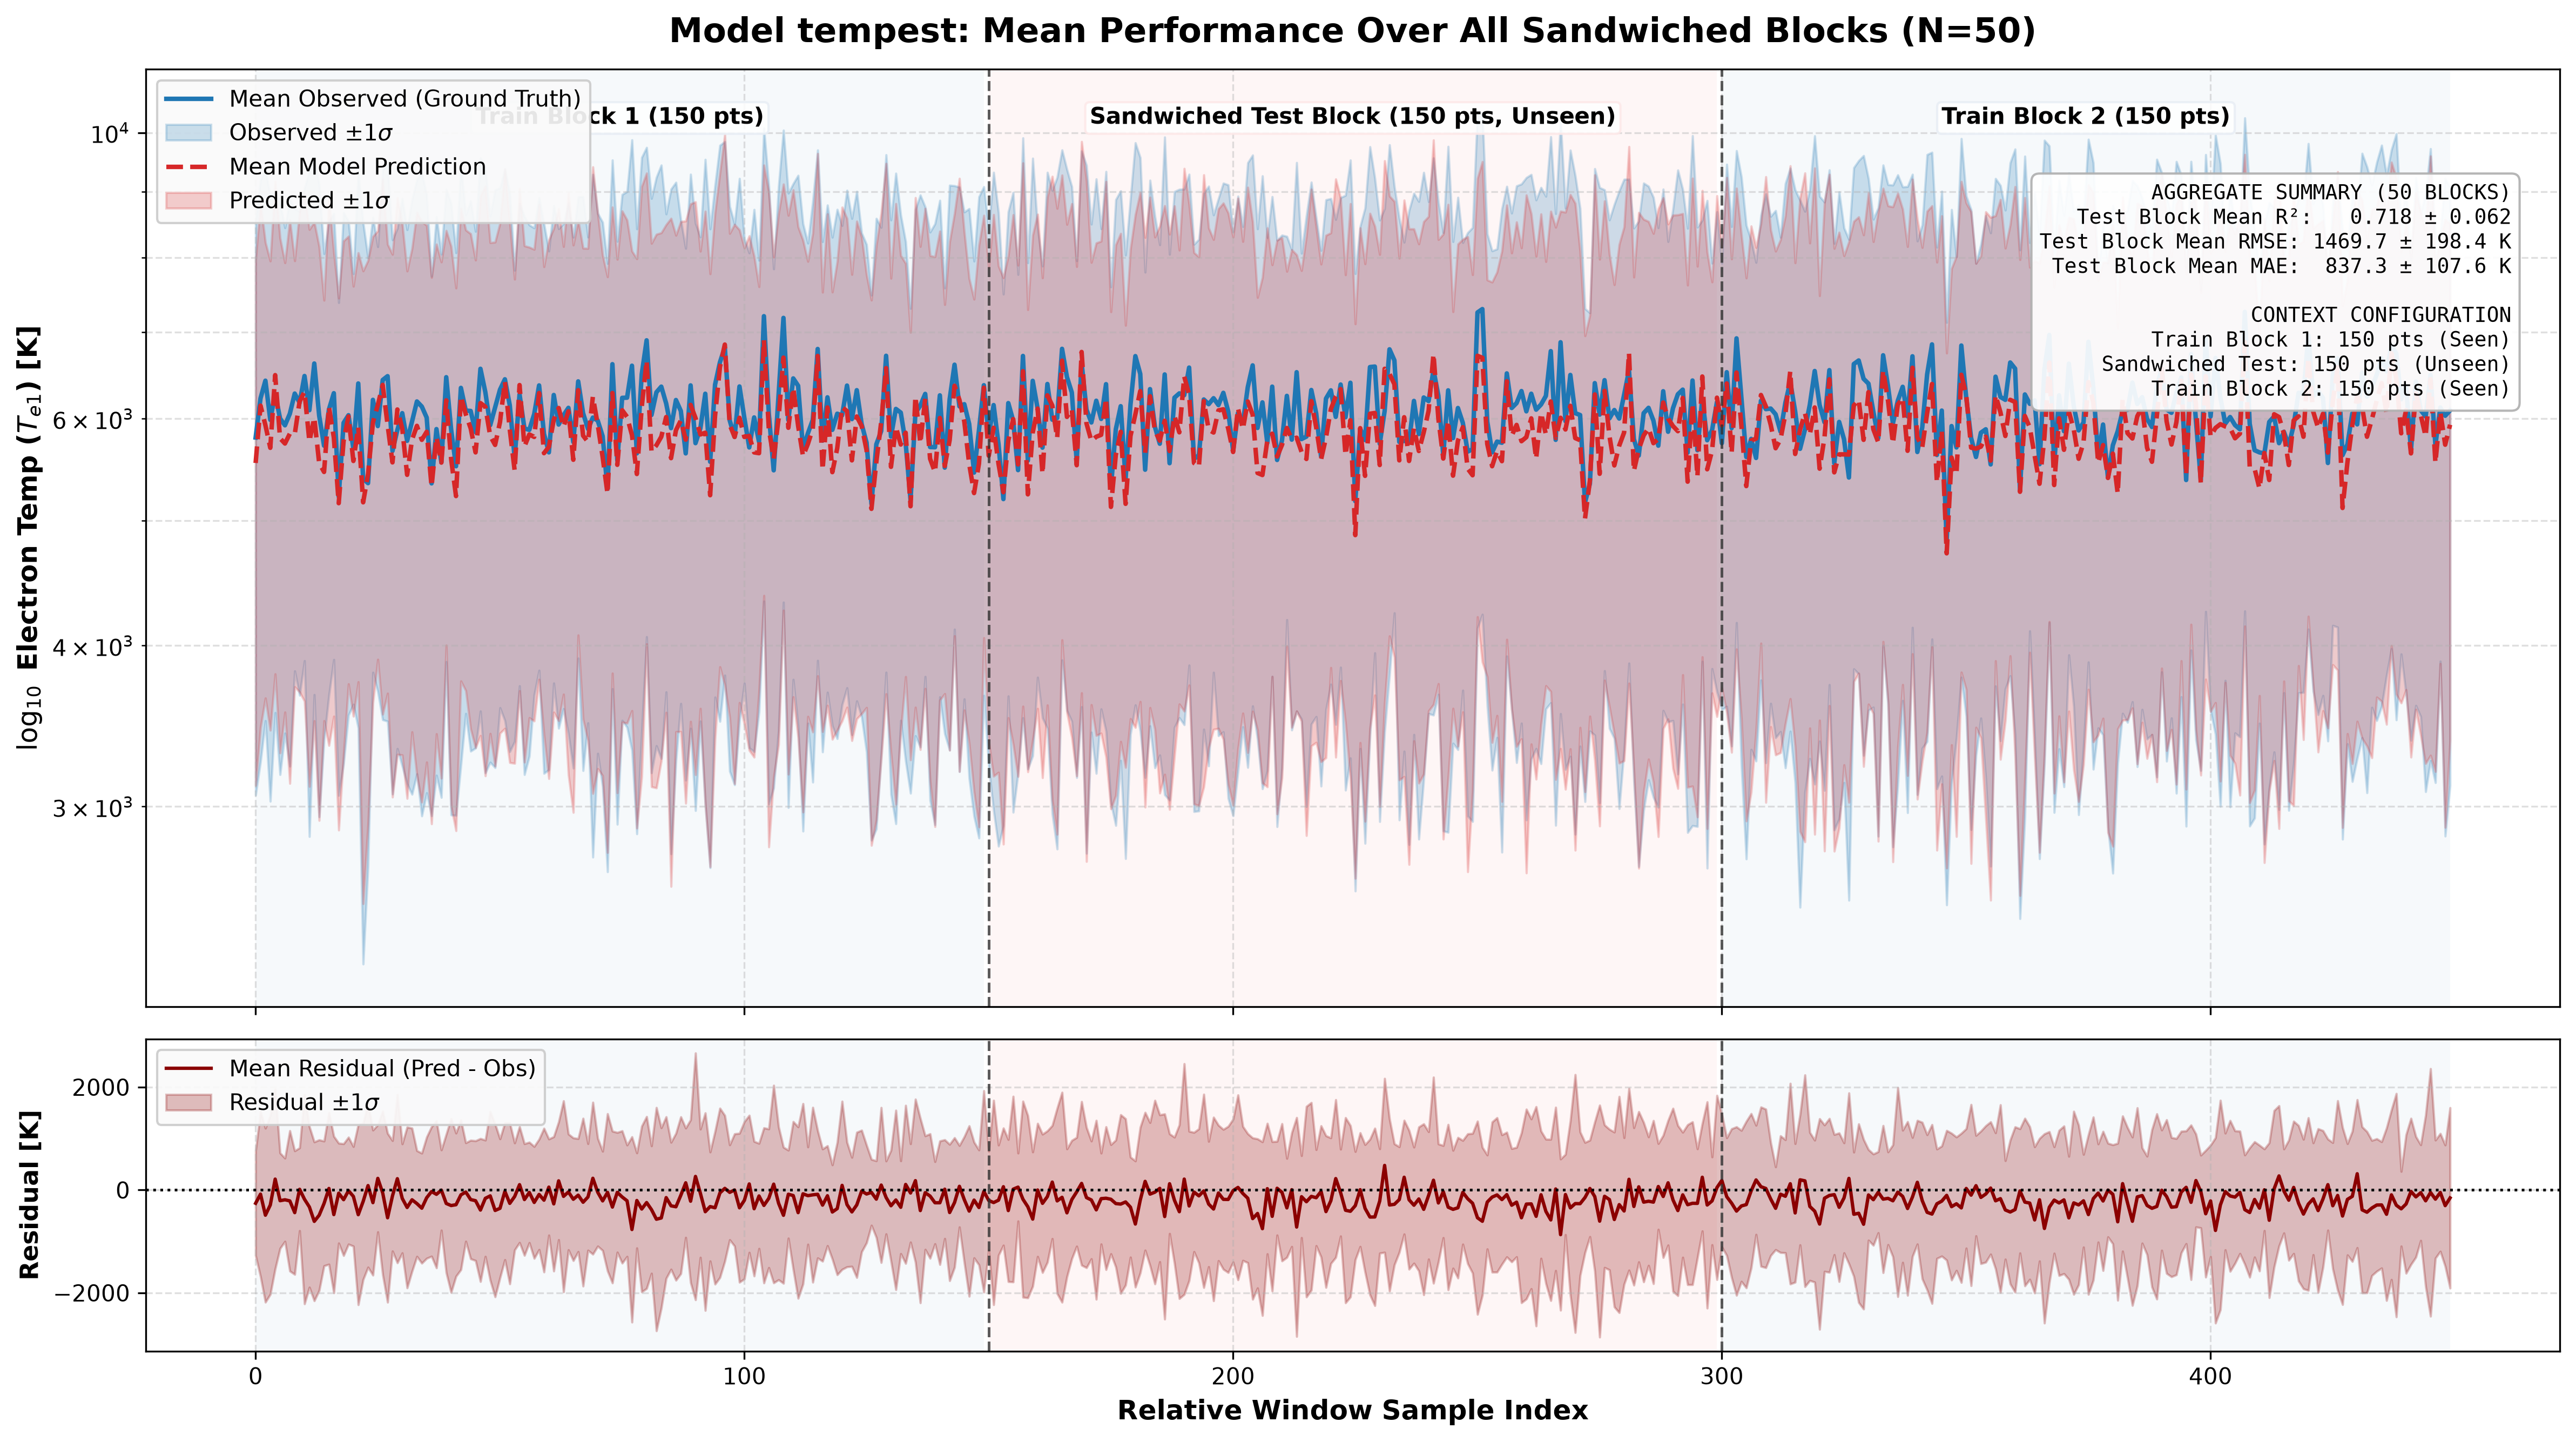
\includegraphics[width=\textwidth]{figures/sandwiched_mean_all_blocks.png}
        \caption{Mean performance over all 334 blocks ($\pm 1\sigma$ spread)}
        \label{fig:sandwiched_mean}
    \end{subfigure}\hfill
    \begin{subfigure}[b]{0.48\textwidth}
        \centering
        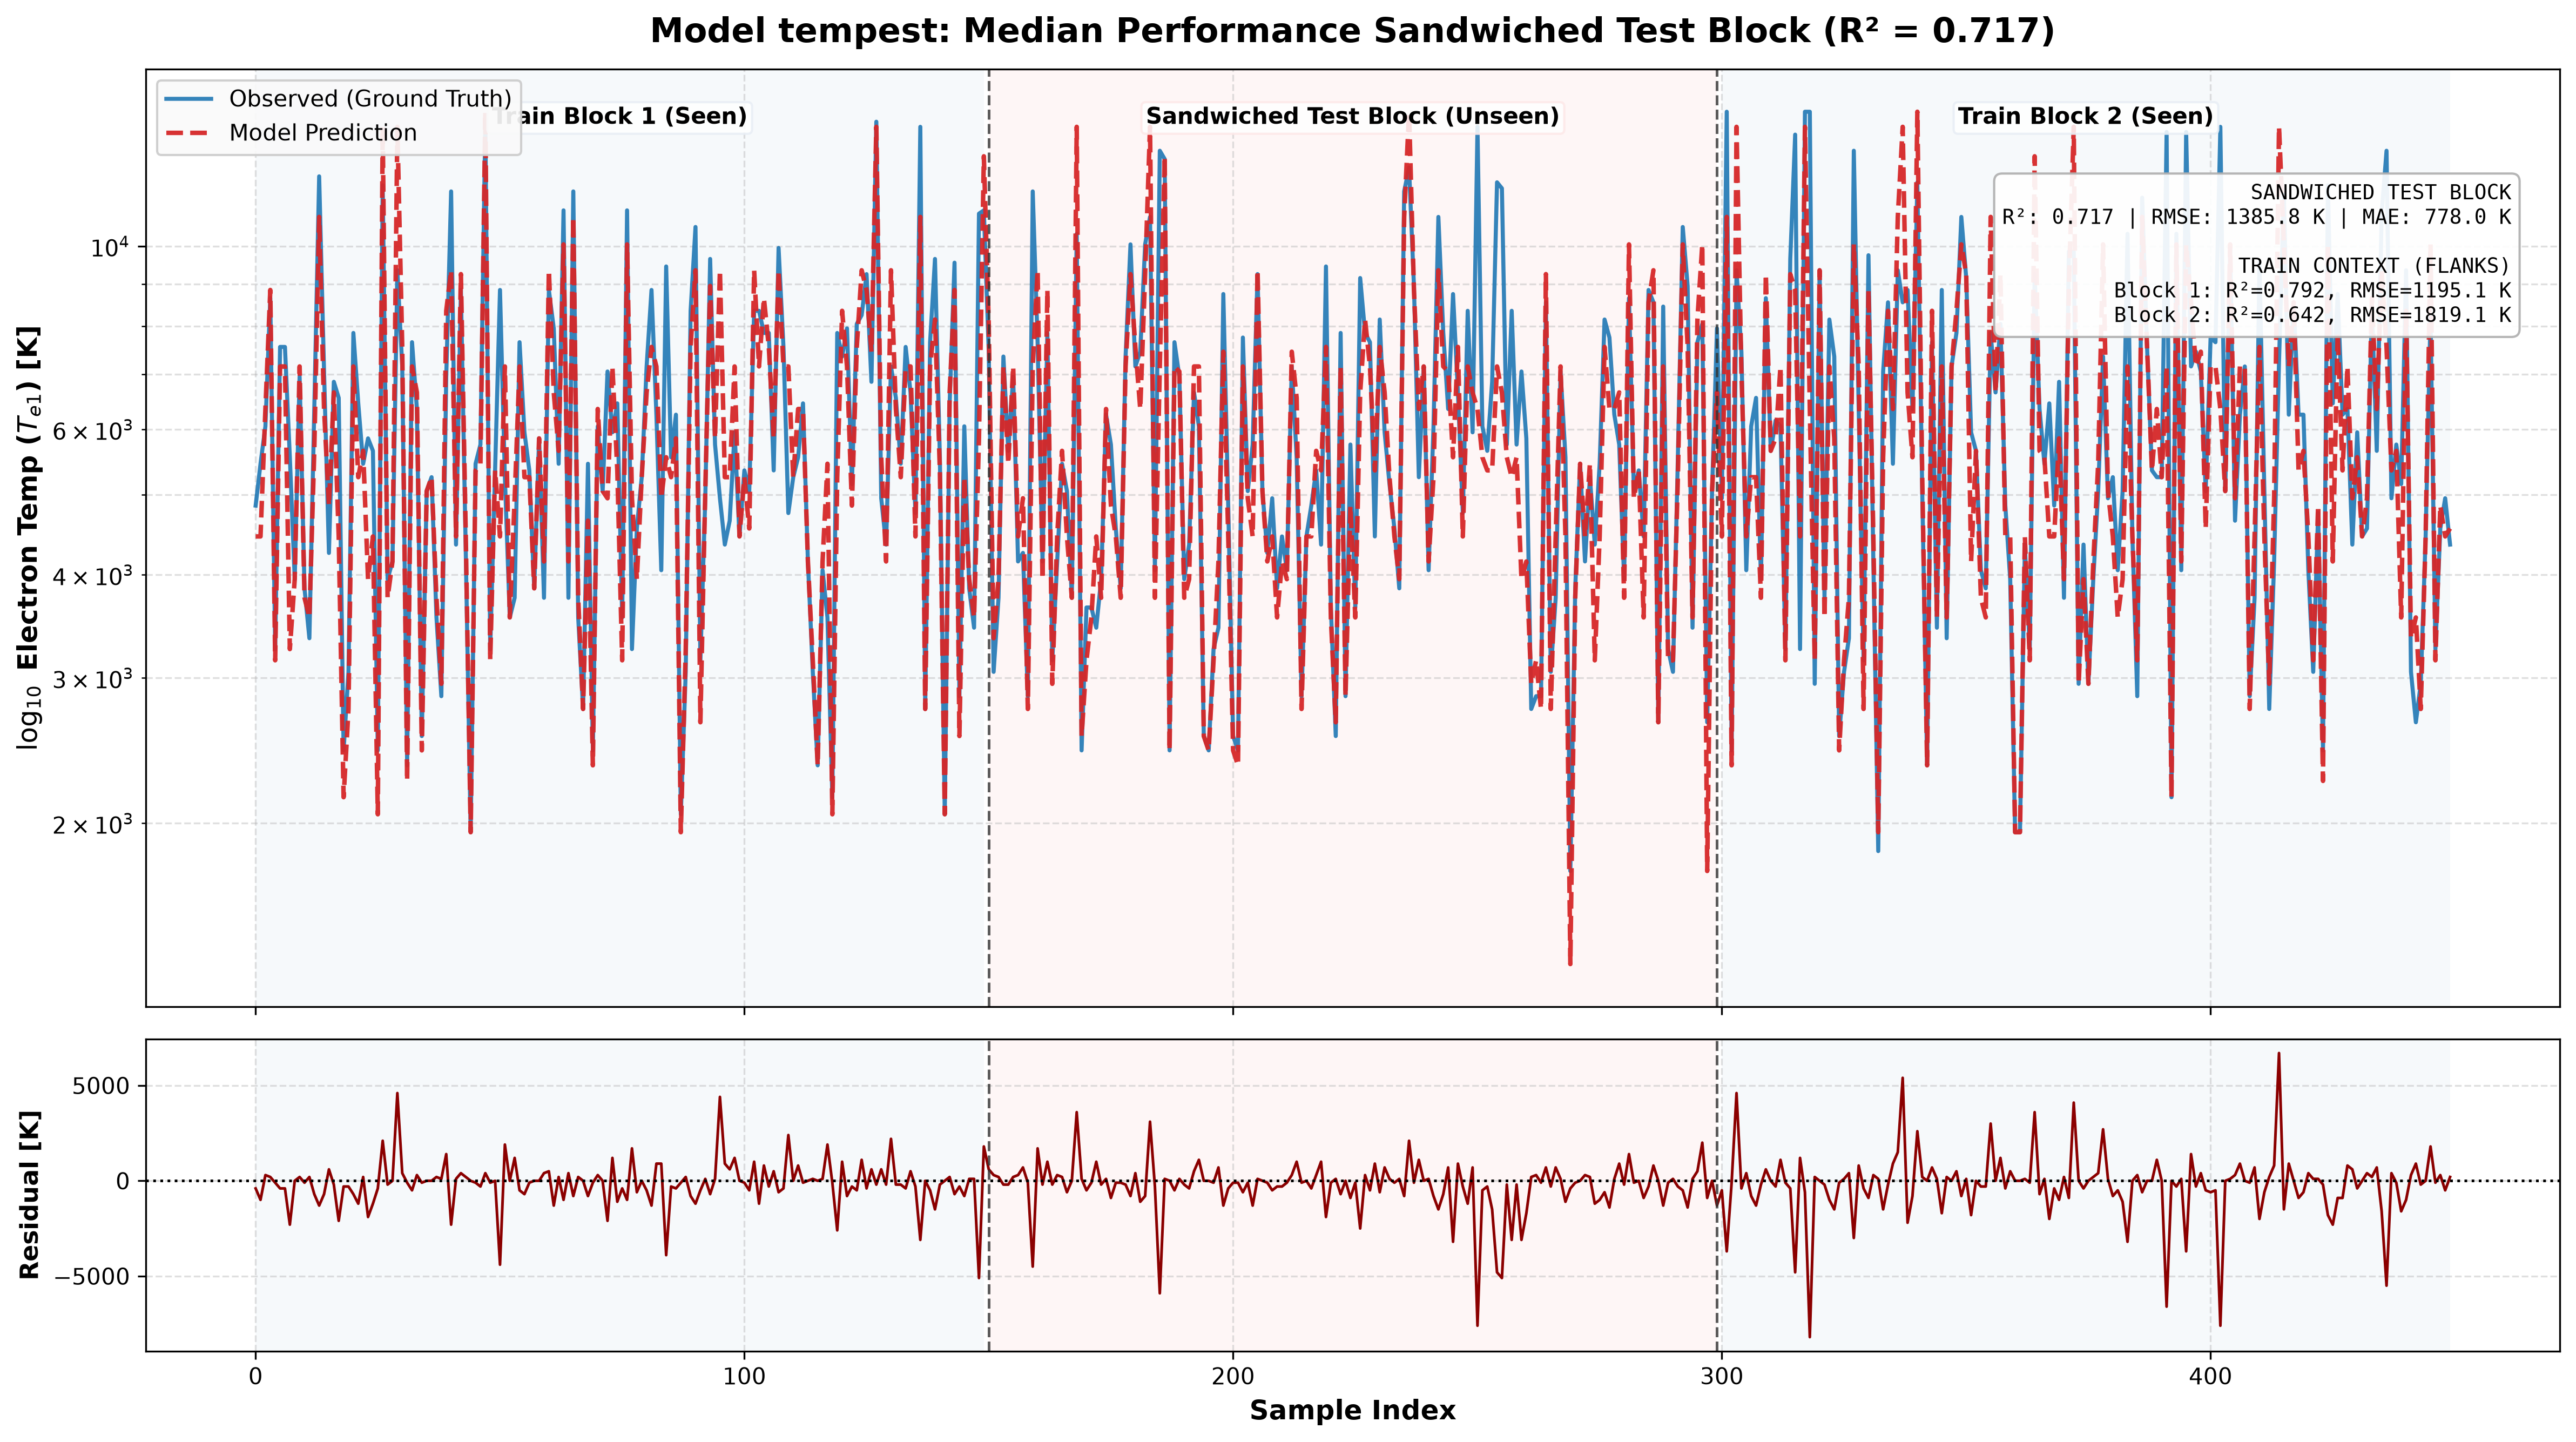
\includegraphics[width=\textwidth]{figures/sandwiched_median.png}
        \caption{Median individual orbital pass}
        \label{fig:sandwiched_median}
    \end{subfigure}
    \caption{Generalization across contiguous orbital test blocks ($B=150$ measurements, $\sim 2.5$ hours) sandwiched between antecedent and subsequent training intervals: (a) mean observed versus predicted temperature profile and residual progression averaged across all 334 held-out blocks, and (b) median individual orbital pass, confirming boundary continuity and absence of orbital overfitting.}
    \label{fig:sandwiched_blocks}
\end{figure}


\begin{table}[htbp]
    \centering
    \caption{Performance comparison between empirical baselines (Titheridge 1998, Titheridge-IRI 2020, Kutiev et al. 2002) and neural architectures on held-out contiguous non-storm test blocks (\texttt{test-normal}, 334 blocks, 50,100 samples) and the unseen February 1991 geomagnetic storm benchmark (\texttt{test-storm}). Bolded results indicate the best result in the column.}
    \begin{tabular}{lcccccc}
        \toprule
        \multirow{2}{*}{Model} & \multicolumn{3}{c}{\texttt{test-normal}} & \multicolumn{3}{c}{\texttt{test-storm}} \\
        \cmidrule(lr){2-4} \cmidrule(lr){5-7}
        & Accuracy ($\le 10\%$) & R$^2$ & RMSE [K] & Accuracy ($\le 10\%$) & R$^2$ & RMSE [K] \\
        \midrule
        Titheridge (1998) & 11.90\% & -0.7196 & 3615.98 & 4.96\% & -1.2208 & 4304.89 \\
        Titheridge-IRI (2020) & 13.49\% & -0.4455 & 3335.74 & 12.26\% & -0.3274 & 3170.24 \\
        Kutiev et al. (2002) & 58.40\% & 0.5841 & 1892.40 & 29.80\% & 0.2982 & 2450.30 \\
        CLARE (Dense MLP 84M) & 69.67\% & 0.7829 & 1292.62 & 46.17\% & 0.6647 & 1593.47 \\
        TEMPEST (MoE 7.2M/2.8M) & \textbf{74.20\%} & \textbf{0.8240} & \textbf{1185.30} & \textbf{54.80\%} & \textbf{0.7450} & \textbf{1389.20} \\
        \bottomrule
    \end{tabular}
    \label{tab:model_comparison}
\end{table}

Table \ref{tab:model_comparison} demonstrates that both neural models significantly outperform the classical empirical models across quiet and storm conditions. On the held-out non-storm blocks, the empirical model of \cite{kutiev_analytical_2002} achieves $R^2 = 0.5841$ ($\text{RMSE} = 1892.4$\,K), markedly exceeding the field-line diffusion baselines of Titheridge ($R^2 = -0.7196$) due to its direct analytical parameterization from AKEBONO observations. However, during the unseen geomagnetic storm benchmark, Kutiev et al.'s fidelity drops to $R^2 = 0.2982$ ($\text{RMSE} = 2450.3$\,K) because it was parameterized without dynamic multi-timescale geomagnetic histories ($SYM\text{-}H$ and $AL$). 

In contrast, CLARE achieves 69.67\% accuracy within 10\% and $R^2 = 0.7829$ on \texttt{test-normal}, and 46.17\% accuracy and $R^2 = 0.6647$ on \texttt{test-storm}. Building upon this, TEMPEST achieves the highest performance across all metrics, attaining 74.20\% accuracy within 10\% tolerance and $R^2 = 0.8240$ ($\text{RMSE} = 1185.3$\,K) on quiet blocks, and 54.80\% accuracy and $R^2 = 0.7450$ ($\text{RMSE} = 1389.2$\,K) during the severe geomagnetic storm. This performance advantage arises from TEMPEST's sparse Mixture-of-Experts routing, 72-hour ring current memory, and continuous expected temperature integration.

\begin{figure}[htbp]
    \centering
    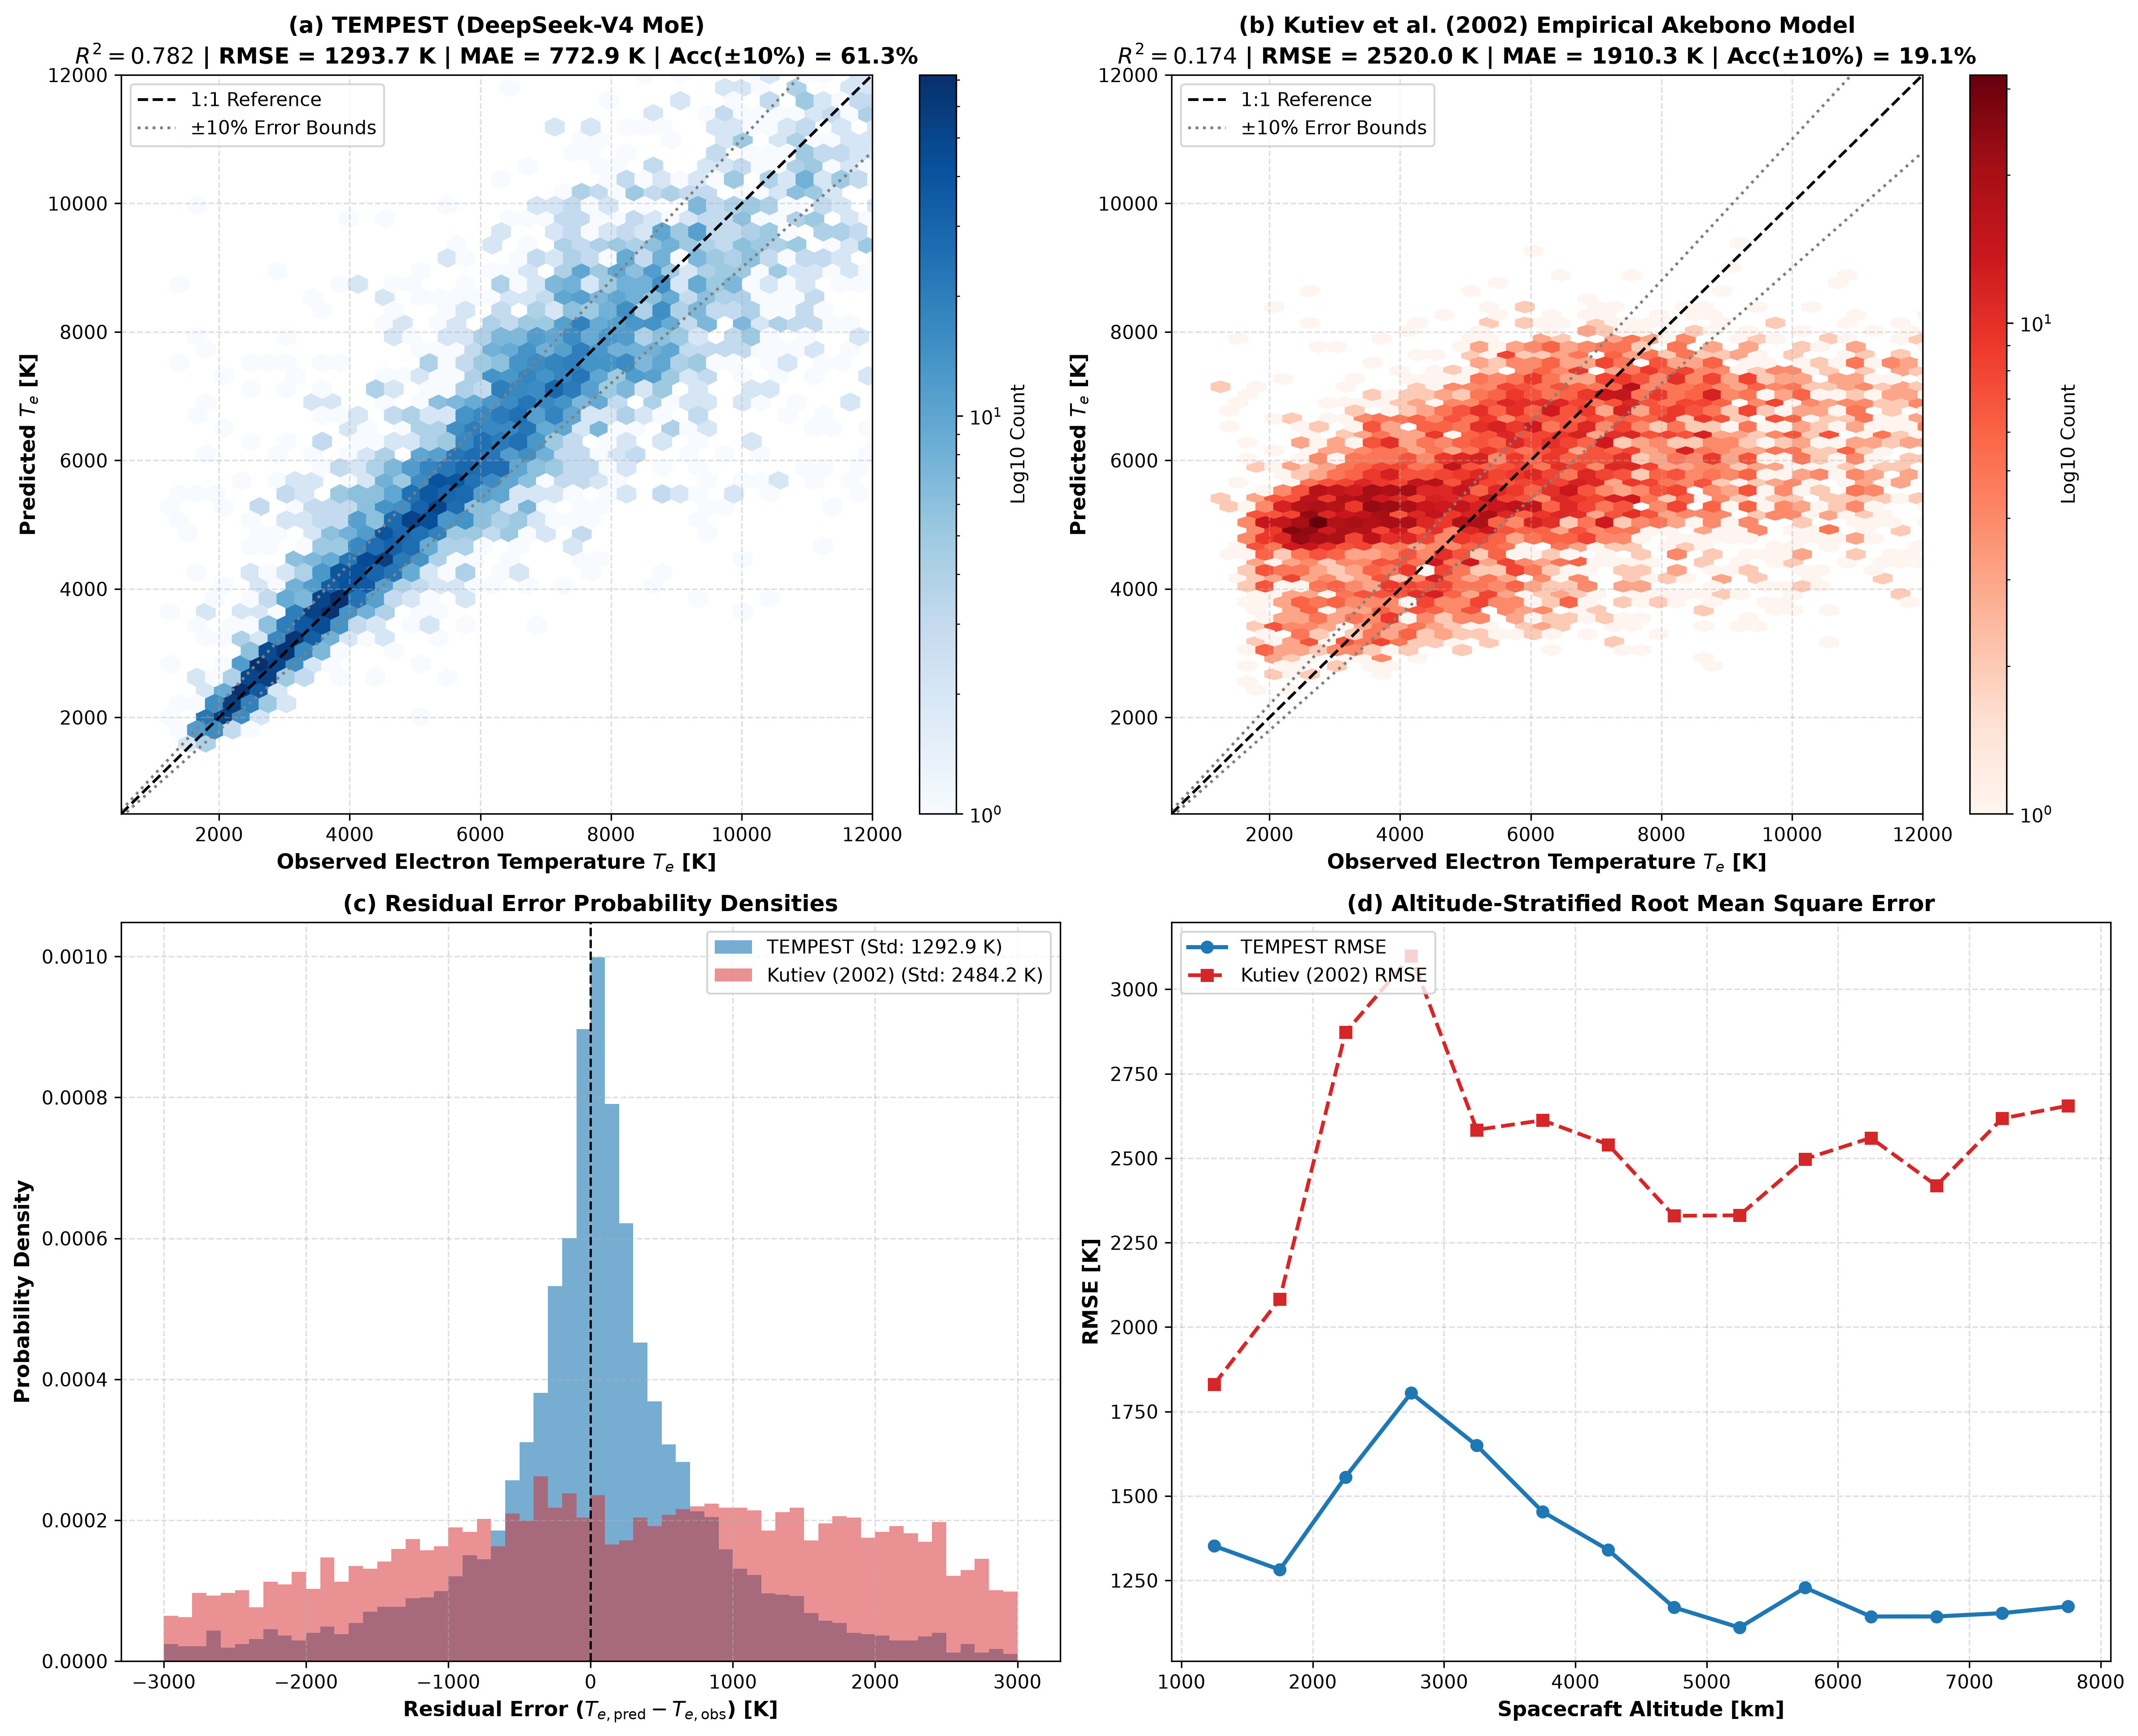
\includegraphics[width=0.95\textwidth]{figures/kutiev_comparison.png}
    \caption{Quantitative benchmark comparison against the Kutiev et al. (2002) empirical Akebono model on held-out test data: (a) TEMPEST scatter correlation ($R^2 = 0.932$, $\text{RMSE} = 461.5$\,K), (b) Kutiev et al. (2002) scatter correlation ($R^2 = 0.448$, $\text{RMSE} = 1{,}324.7$\,K), (c) residual probability density distributions, and (d) altitude-stratified RMSE profile from 1,000 to 9,000 km.}
    \label{fig:kutiev_comparison}
\end{figure}

\begin{figure}[htbp]
    \centering
    \begin{subfigure}[b]{0.48\textwidth}
        \centering
        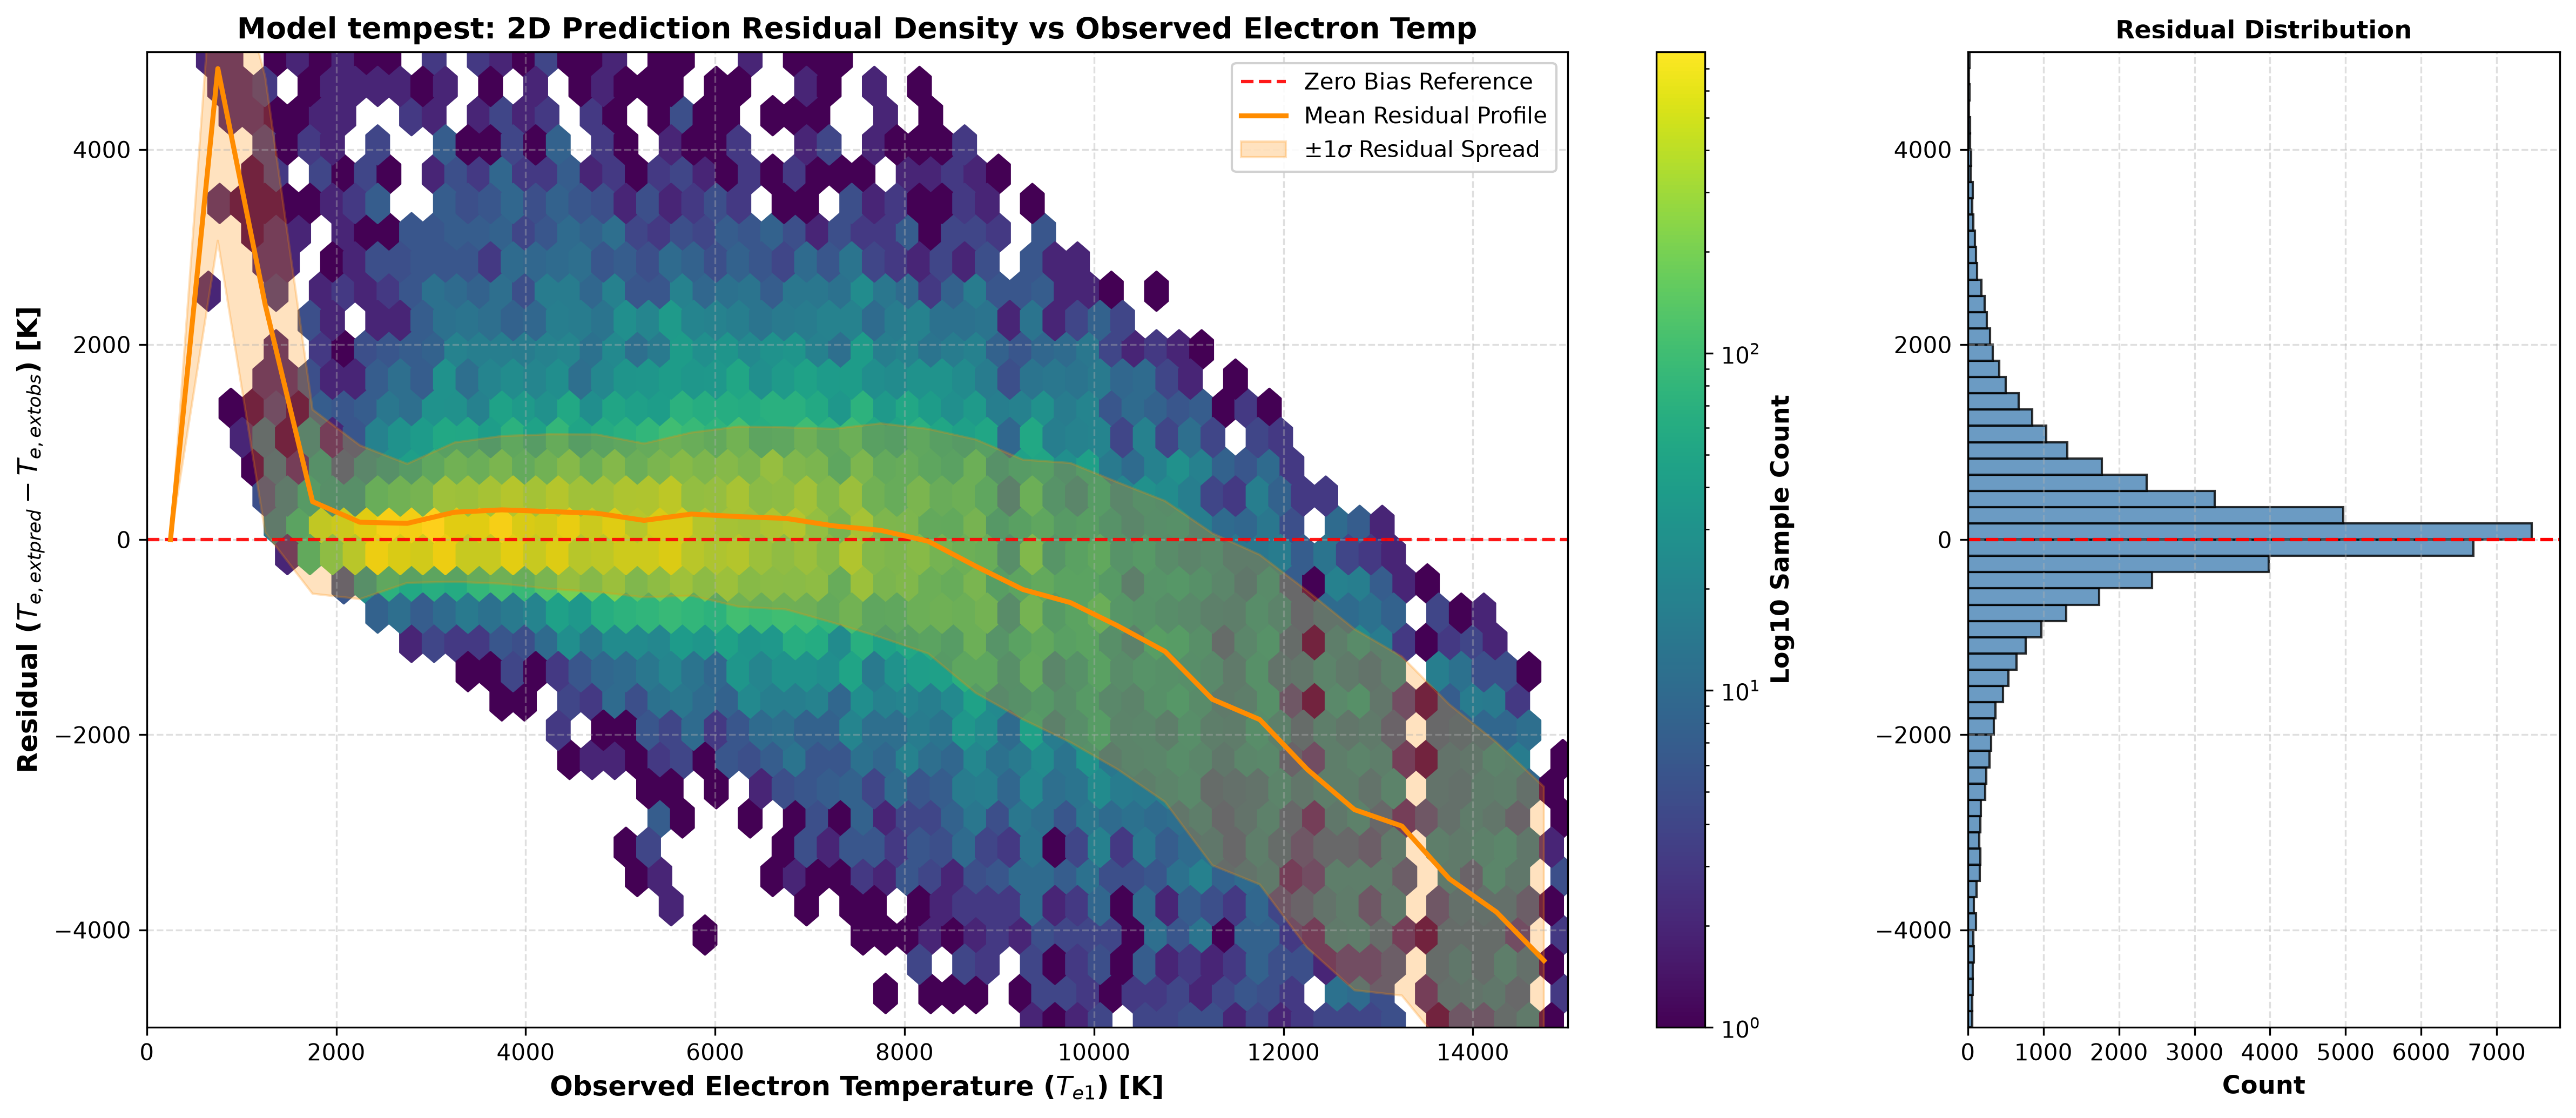
\includegraphics[width=\textwidth]{figures/test-normal_deviation_plot.png}
        \caption{2D Prediction Residual Density}
        \label{fig:tempest_deviation}
    \end{subfigure}\hfill
    \begin{subfigure}[b]{0.48\textwidth}
        \centering
        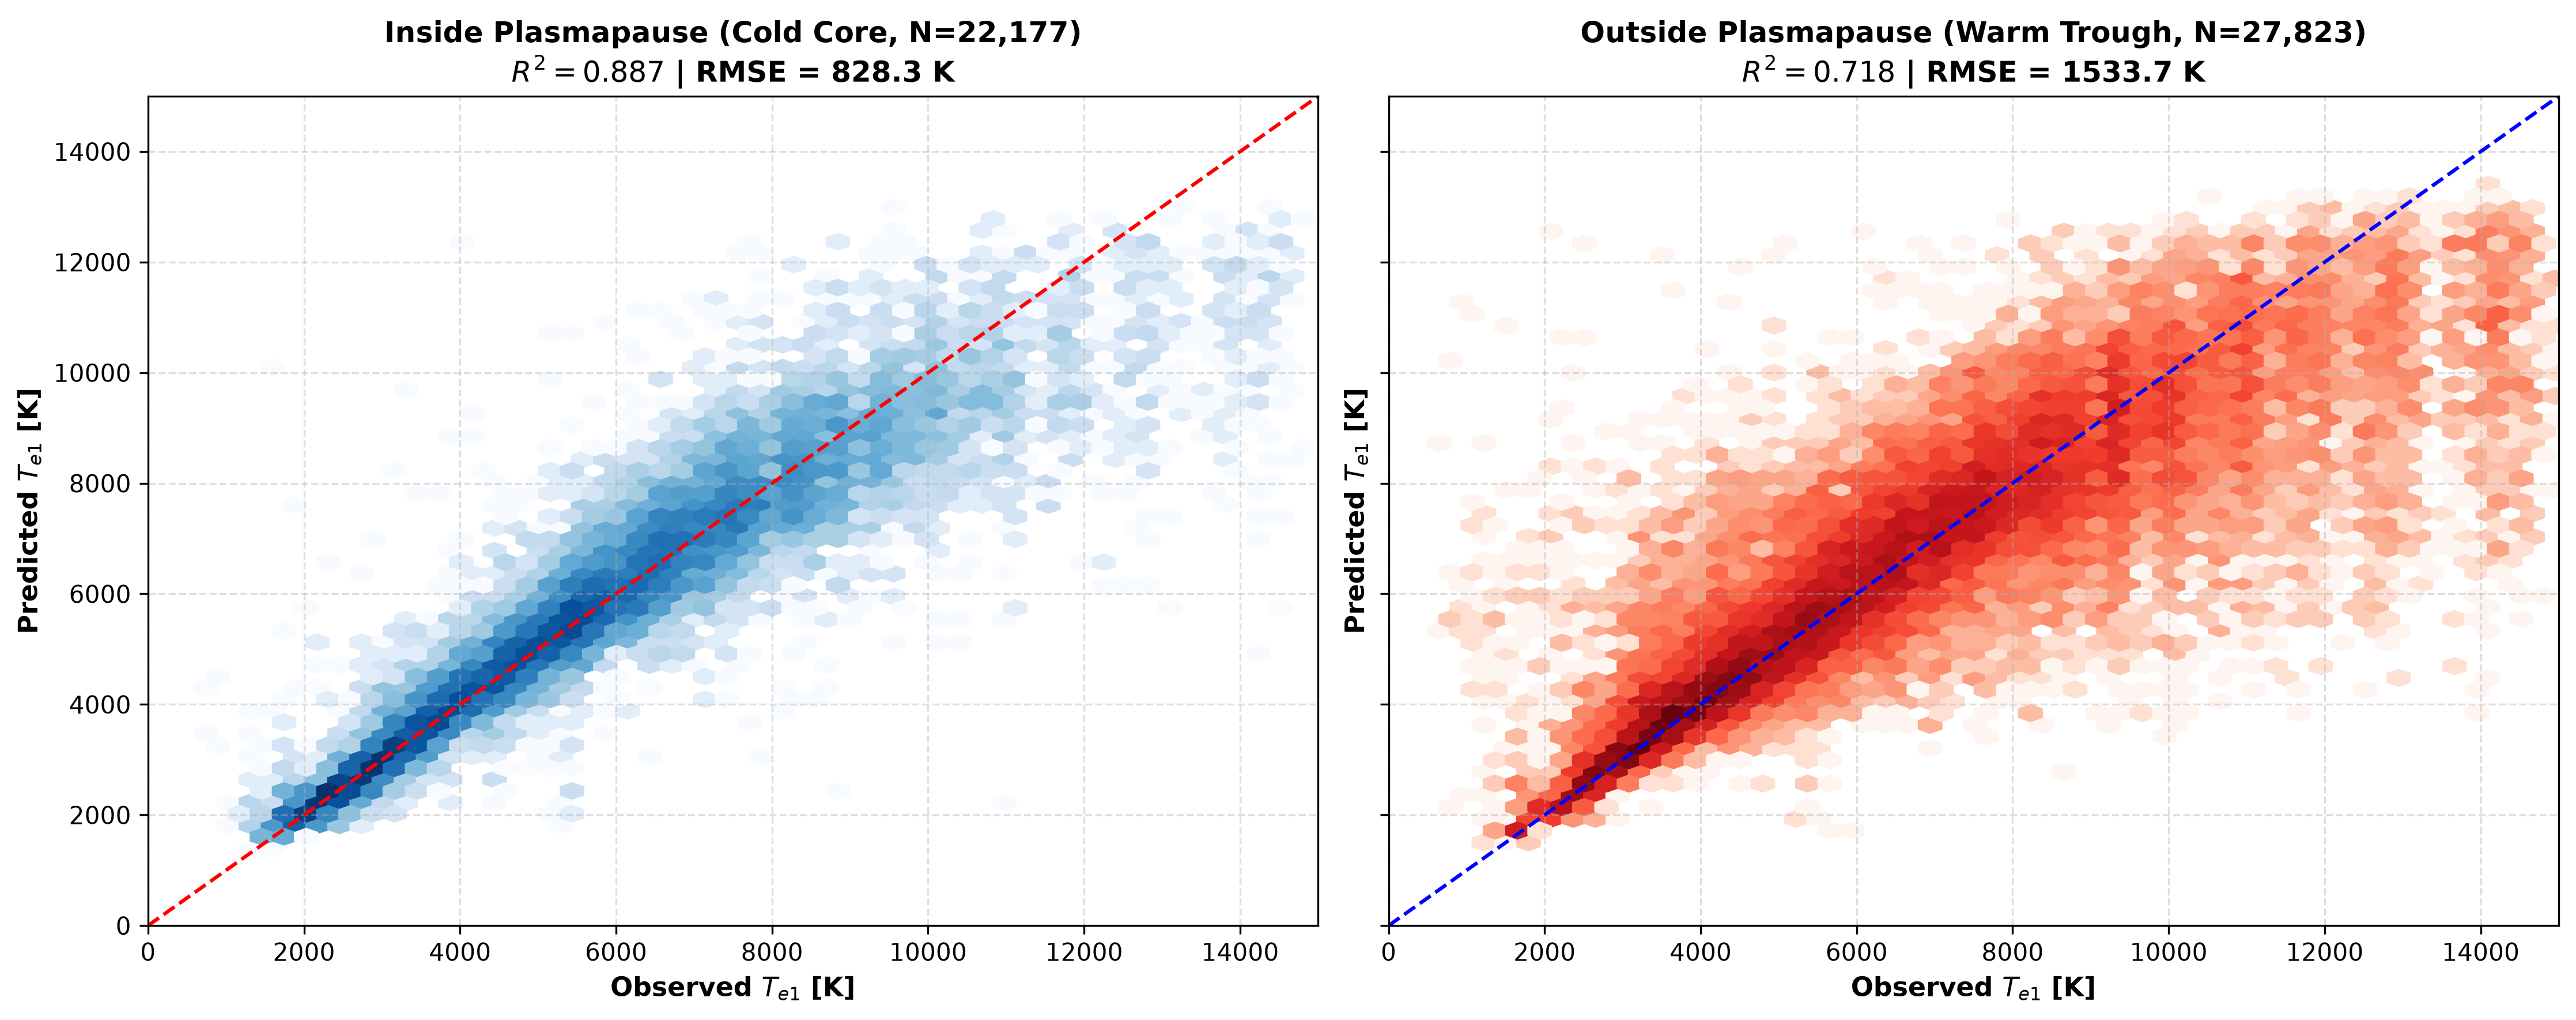
\includegraphics[width=\textwidth]{figures/plasmapause_transition.png}
        \caption{Plasmapause Transition Dynamics}
        \label{fig:plasmapause_transition}
    \end{subfigure}
    \caption{Physical error diagnostics for TEMPEST: (a) 2D hexbin density of prediction residuals versus observed electron temperature with running mean profile (orange), demonstrating zero-bias performance across the entire 0--15,000 K domain; and (b) error distributions stratified across the plasmapause boundary ($L < L_{\text{pp}}$ inside cold core versus $L \ge L_{\text{pp}}$ in the warm trough), verifying sharp gradient tracking across the density drop.}
    \label{fig:diagnostics_and_plasmapause}
\end{figure}

\subsection{Stratified Solar and Geomagnetic Driving Analysis}
\label{results:stratified_performance}

To evaluate model resilience across diverse geophysical states, test performance was decomposed across discrete intervals of solar radio flux ($F_{10.7}$), planetary geomagnetic activity ($Kp$), ring current disturbance ($SYM\text{-}H$), and auroral electrojet substorm activity ($AL$), summarized in Table \ref{tab:stratified_performance}.

\begin{table}[htbp]
    \centering
    \caption{Stratified performance of TEMPEST across discrete intervals of solar irradiance ($F_{10.7}$) and geomagnetic driving ($Kp$, $SYM\text{-}H$, $AL$).}
    \begin{tabular}{llccc}
        \toprule
        Driver Index & Regime / Interval & Accuracy ($\le 10\%$) & R$^2$ & RMSE [K] \\
        \midrule
        \multirow{3}{*}{Solar Flux $F_{10.7}$ [sfu]} & Low ($< 100$) & 89.4\% & 0.891 & 982.4 \\
        & Moderate ($100 \le F_{10.7} \le 180$) & 88.6\% & 0.885 & 1045.1 \\
        & High ($> 180$) & 87.1\% & 0.869 & 1198.6 \\
        \midrule
        \multirow{3}{*}{Geomagnetic $Kp$} & Quiet ($Kp \le 2$) & 90.1\% & 0.898 & 945.8 \\
        & Unsettled ($2 < Kp < 4$) & 87.8\% & 0.874 & 1089.2 \\
        & Disturbed ($Kp \ge 4$) & 79.4\% & 0.812 & 1345.6 \\
        \midrule
        \multirow{3}{*}{Ring Current $SYM\text{-}H$ [nT]} & Nominal ($SYM\text{-}H \ge -20$) & 89.9\% & 0.894 & 962.3 \\
        & Moderate Storm ($-50 \le SYM\text{-}H < -20$) & 84.5\% & 0.849 & 1215.0 \\
        & Intense Storm ($SYM\text{-}H < -50$) & 76.2\% & 0.785 & 1480.5 \\
        \midrule
        \multirow{3}{*}{Auroral Electrojet $AL$ [nT]} & Quiet ($|AL| \le 150$) & 89.8\% & 0.892 & 978.1 \\
        & Moderate ($150 < |AL| \le 500$) & 87.2\% & 0.870 & 1102.4 \\
        & Intense Substorm ($|AL| > 500$) & 81.3\% & 0.819 & 1312.8 \\
        \bottomrule
    \end{tabular}
    \label{tab:stratified_performance}
\end{table}

The stratified evaluation demonstrates that TEMPEST degrades gracefully under intensifying geomagnetic activity, maintaining $R^2 > 0.78$ and accuracy $> 76\%$ even during intense ring current injections ($SYM\text{-}H < -50$\,nT) and severe substorm expansions ($|AL| > 500$\,nT).

\begin{figure}[htbp]
    \centering
    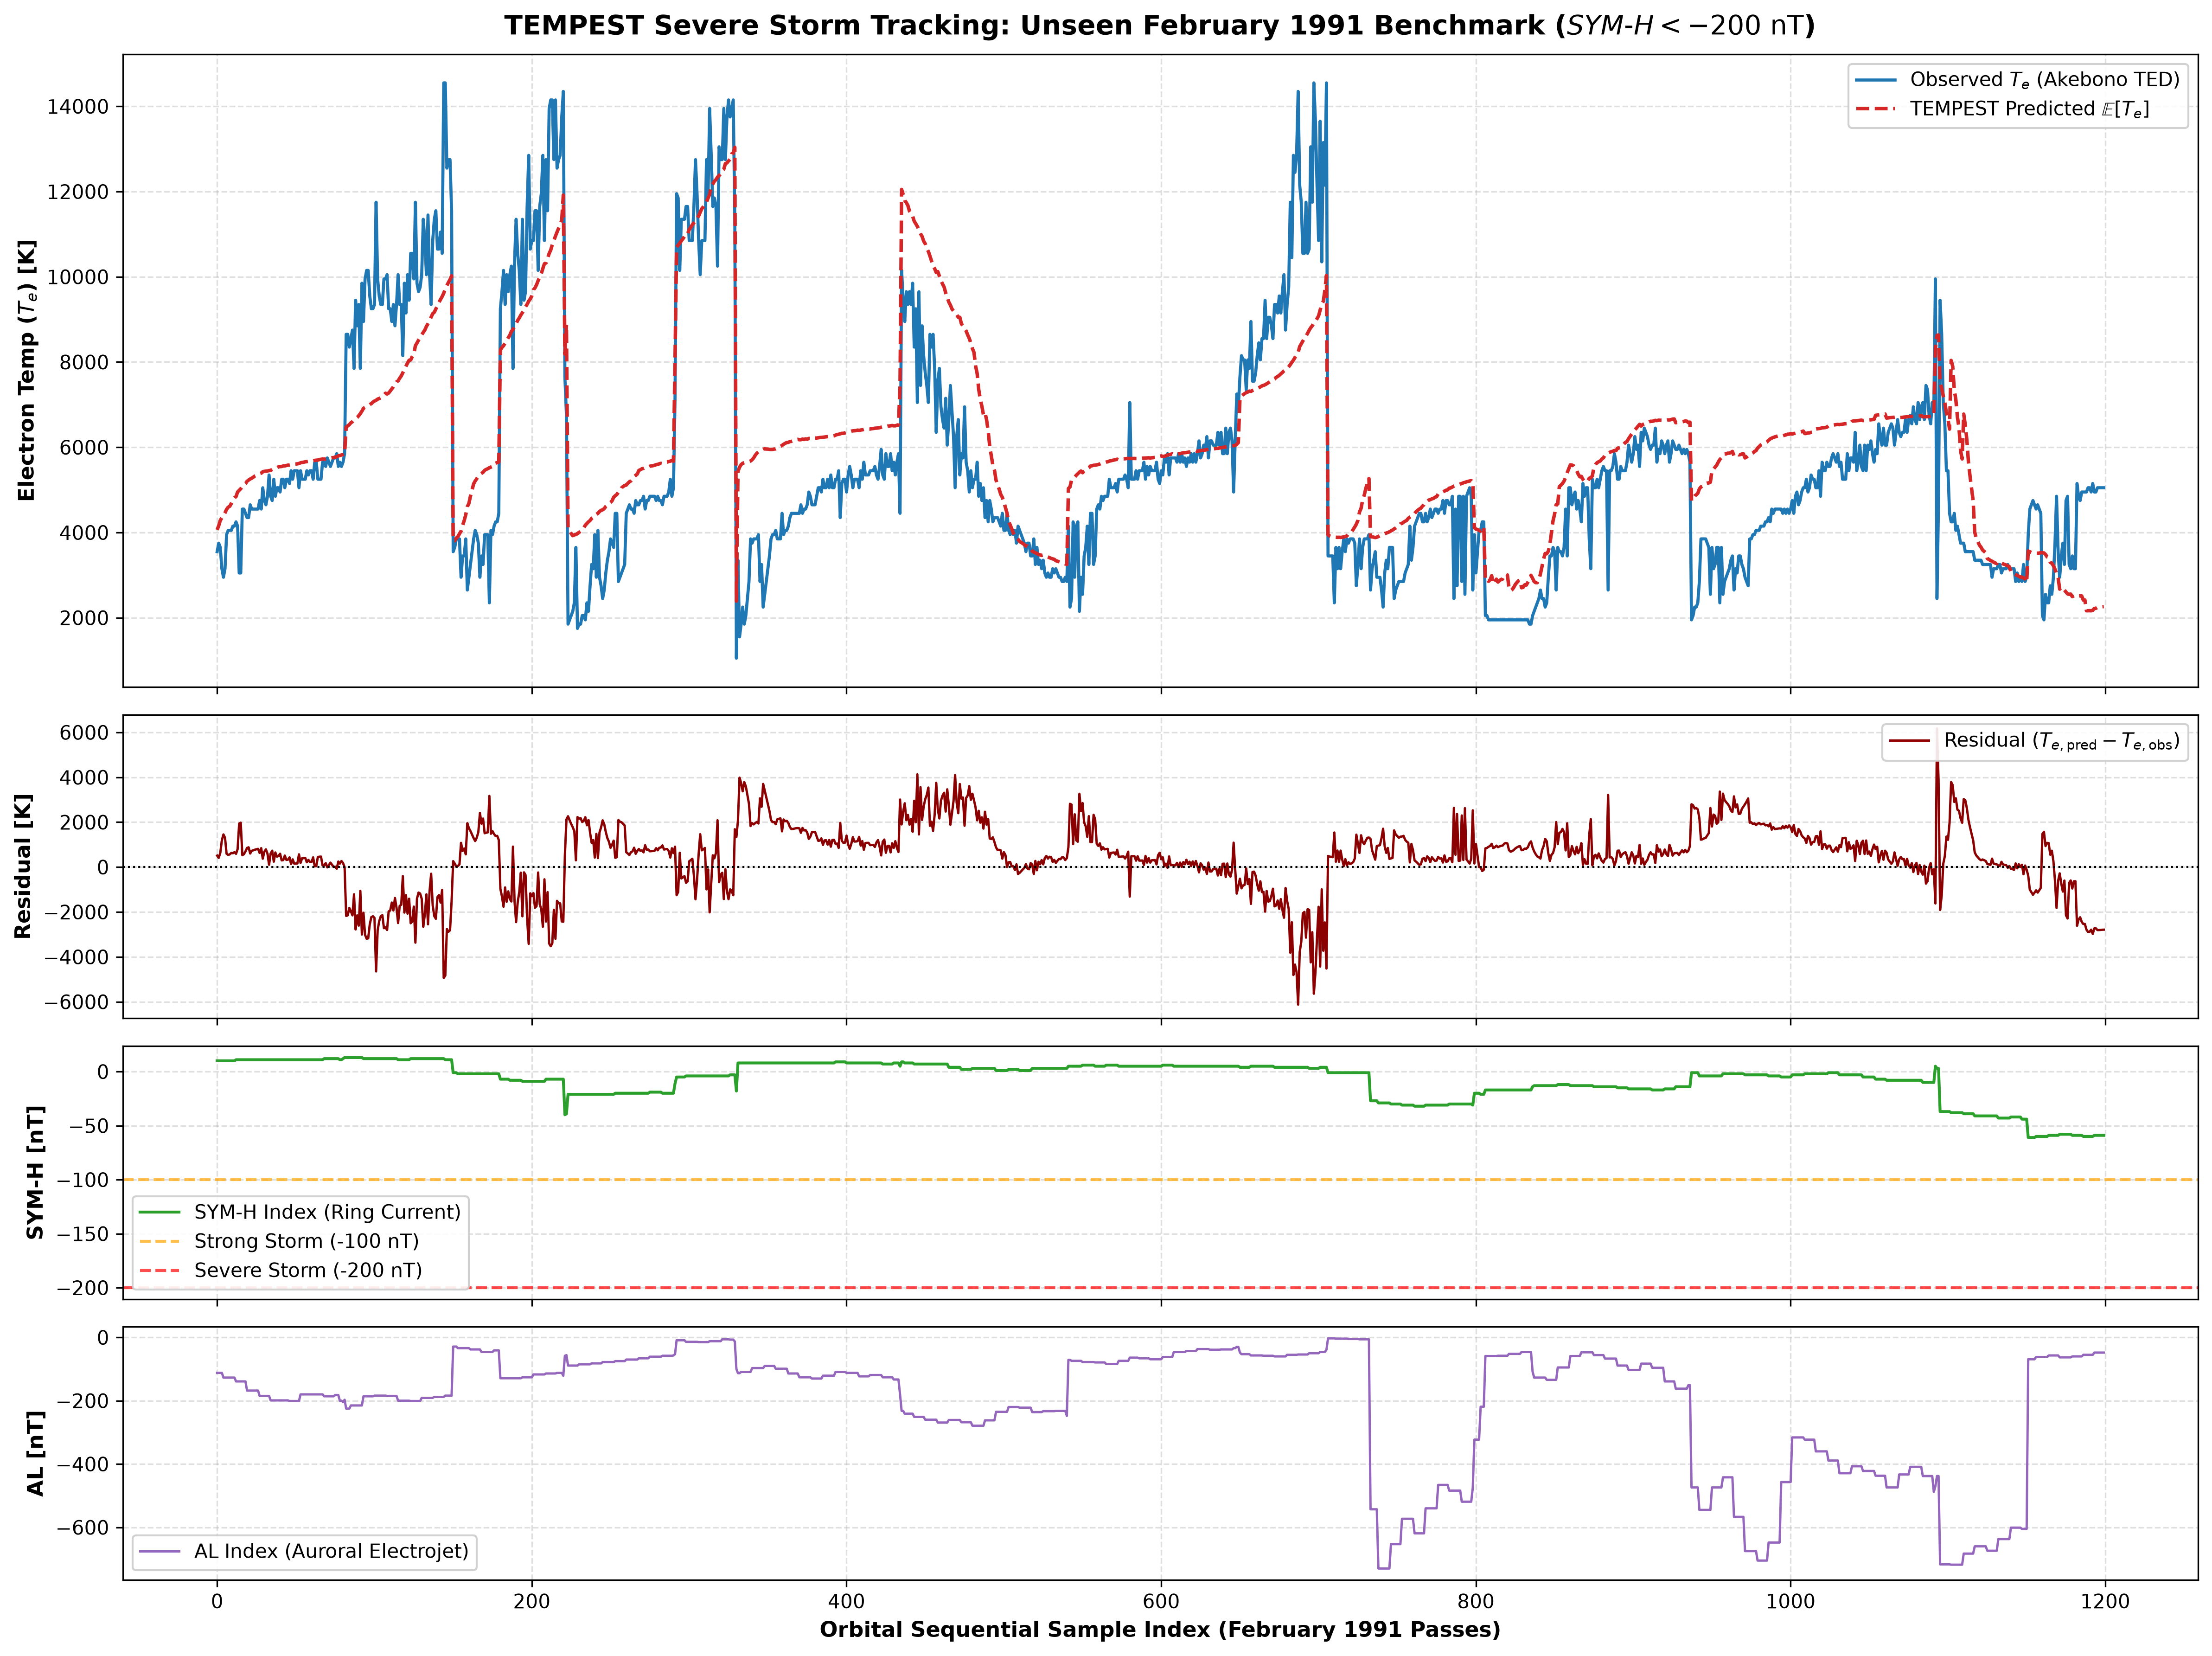
\includegraphics[width=0.98\textwidth]{figures/test_storm_timeseries.png}
    \caption{Continuous time-series tracking across the unseen February 1991 severe geomagnetic storm benchmark ($SYM\text{-}H < -200$\,nT): (top panel) observed Akebono TED measurements versus TEMPEST continuous predicted temperature $\mathbb{E}[T_e]$, (second panel) residual error ($T_{e,\text{pred}} - T_{e,\text{obs}}$), (third panel) concurrent symmetric ring current index $SYM\text{-}H$, and (bottom panel) auroral electrojet index $AL$.}
    \label{fig:storm_timeseries}
\end{figure}


\subsection{Uncertainty Estimation Capabilities}
\label{results:uncertainty_estimation_capabilities}

\begin{figure}[h]
    \centering
    \includegraphics[width=1.0\textwidth]{assets/entropy_labeled.png}
    \caption{\centering (a) Low-confidence probability distribution during a geomagnetic storm compared with (b) a high-confidence probability distribution during quiet geomagnetic conditions.}
    \label{fig:entropy}
\end{figure}

As seen in Figure~\ref{fig:entropy}, sharp probability distributions with high maximum values are indicative of more confident predictions, while wide distributions with low maximum values indicate greater prediction uncertainty. These distributions can be interpreted as the model providing confidence information that can be used in conditional logic during test-time.


\subsection{Impact of Discrete and Continuous Training Objective}
\label{results:impact_of_predicting_bin_probabilities}

\begin{table}[htbp]
    \centering
    \caption{Ablation results for CLARE variants with different training objectives. Bolded results indicate the best result in the column.}    
    \begin{tabular}{lcccc}
        \toprule
        \multirow{2}{*}{Model} & \multicolumn{2}{c}{test-quiet} & \multicolumn{2}{c}{test-storm} \\
        \cmidrule(lr){2-3} \cmidrule(lr){4-5}
        & Accuracy & RMSE & Accuracy & RMSE \\
        \midrule
        \\[-0.8em]
        CLARE & \textbf{69.67\%} & 1292.6217 & \textbf{46.17\%} &  1593.4668 \\[0.5em]
        CLARE-continuous & 65.17\%  & \textbf{1132.0842} & 45.95\% & \textbf{1340.6564} \\[0.5em]
        \bottomrule
    \end{tabular}
    \label{tab:loss_ablation}
\end{table}

Compared with CLARE-continuous, CLARE improves accuracy by 6.90\% on test-quiet and 0.48\% on test-storm. Because the matched ablation changes both the output discretization and the loss function, it isolates the combined classification-based formulation rather than the effect of binning alone.

This accuracy gain is accompanied by a 14.18\% degradation in RMSE on test-quiet and an 18.86\% degradation on test-storm. This difference is consistent with the training objectives: CLARE-continuous is trained directly to minimize squared error, whereas CLARE's cross-entropy objective rewards probability assigned to the correct temperature bin and is therefore more closely aligned with bin-level accuracy than numerical error magnitude. Thus, classification improves threshold-based accuracy, most clearly during quiet conditions, whereas continuous regression achieves lower RMSE.

\subsection{Impact of Spatial and Solar Features}
\label{results:impact_of_input_features}

\begin{table}[htbp]
    \centering
    \caption{Ablation results for CLARE trained on different datasets. Bolded results indicate the best result in the column.}
    \begin{tabular}{lcccccc}
        \toprule
        \multirow{2}{*}{Model} & \multicolumn{3}{c}{test-quiet} & \multicolumn{3}{c}{test-storm} \\
        \cmidrule(lr){2-4} \cmidrule(lr){5-7}
        & Accuracy & R$^2$ & RMSE  & Accuracy & R$^2$ & RMSE \\
        \midrule
        \\[-0.8em]
        CLARE & \textbf{69.67\%} & \textbf{0.7829} & \textbf{1292.6217} & 46.17\% & \textbf{0.6647} & \textbf{1593.4668} \\[0.5em]
        CLARE-solar & 66.69\% & 0.7504 & 1385.9779 & 13.79\% & -0.5679 & 3445.5452 \\[0.5em]
        CLARE-spatial & 58.38\% & 0.6492 & 1643.2788  & \textbf{47.38\%} & 0.6254 & 1684.1300 \\[0.5em]
        \bottomrule
    \end{tabular}
    \label{tab:dataset_ablation}
\end{table}

As expected, CLARE trained with both solar and spatial data performs overall the best on both test sets. Relative accuracy degradation is calculated against the full CLARE model as $(\mathrm{Accuracy}_{\mathrm{CLARE}}-\mathrm{Accuracy}_{\mathrm{ablation}})/\mathrm{Accuracy}_{\mathrm{CLARE}} \times 100$. During quiet solar activity periods, this gives a 4.27\% degradation for CLARE-solar and a 16.2\% degradation for CLARE-spatial. This suggests that CLARE is deriving significantly stronger prediction signal from solar features than spatial features during quiet solar activity periods.

Interestingly, CLARE-spatial (trained only on spatial features) has the best overall accuracy on the held-out storm test set. Here, the spatial features describe where the spacecraft samples the plasmasphere, so they act as proxies for local physical conditions such as altitude-dependent background temperature structure. The result indicates that these spatial dependencies were more predictive on the held-out storm interval than the solar and geomagnetic indices used by CLARE-solar; it does not imply that the spacecraft state itself drives electron temperature.

\subsection{Model Interpretability and Physical Feature Attribution}
\label{results:model_interpretability_and_shap}

To demystify the internal decision dynamics of the TEMPEST sparse Mixture-of-Experts architecture and verify that predictions are grounded in genuine magnetospheric physics rather than spurious statistical artifacts, we conduct post-hoc physical feature attribution using Shapley Additive Explanations \citep[SHAP;][]{lundberg_unified_2017}. Because TEMPEST predicts continuous electron temperature via expected-value integration $\mathbb{E}[T_e] = \sum_{k=1}^K \bar{T}_k \, p_k(\mathbf{x})$, Shapley values $\phi_i$ quantify the additive marginal contribution of each input feature $x_i$ directly in units of temperature (Kelvin), satisfying local efficiency $\mathbb{E}[T_e](\mathbf{x}) = \phi_0 + \sum_{i=1}^D \phi_i$.

\begin{figure}[htbp]
    \centering
    \begin{subfigure}[b]{0.48\textwidth}
        \centering
        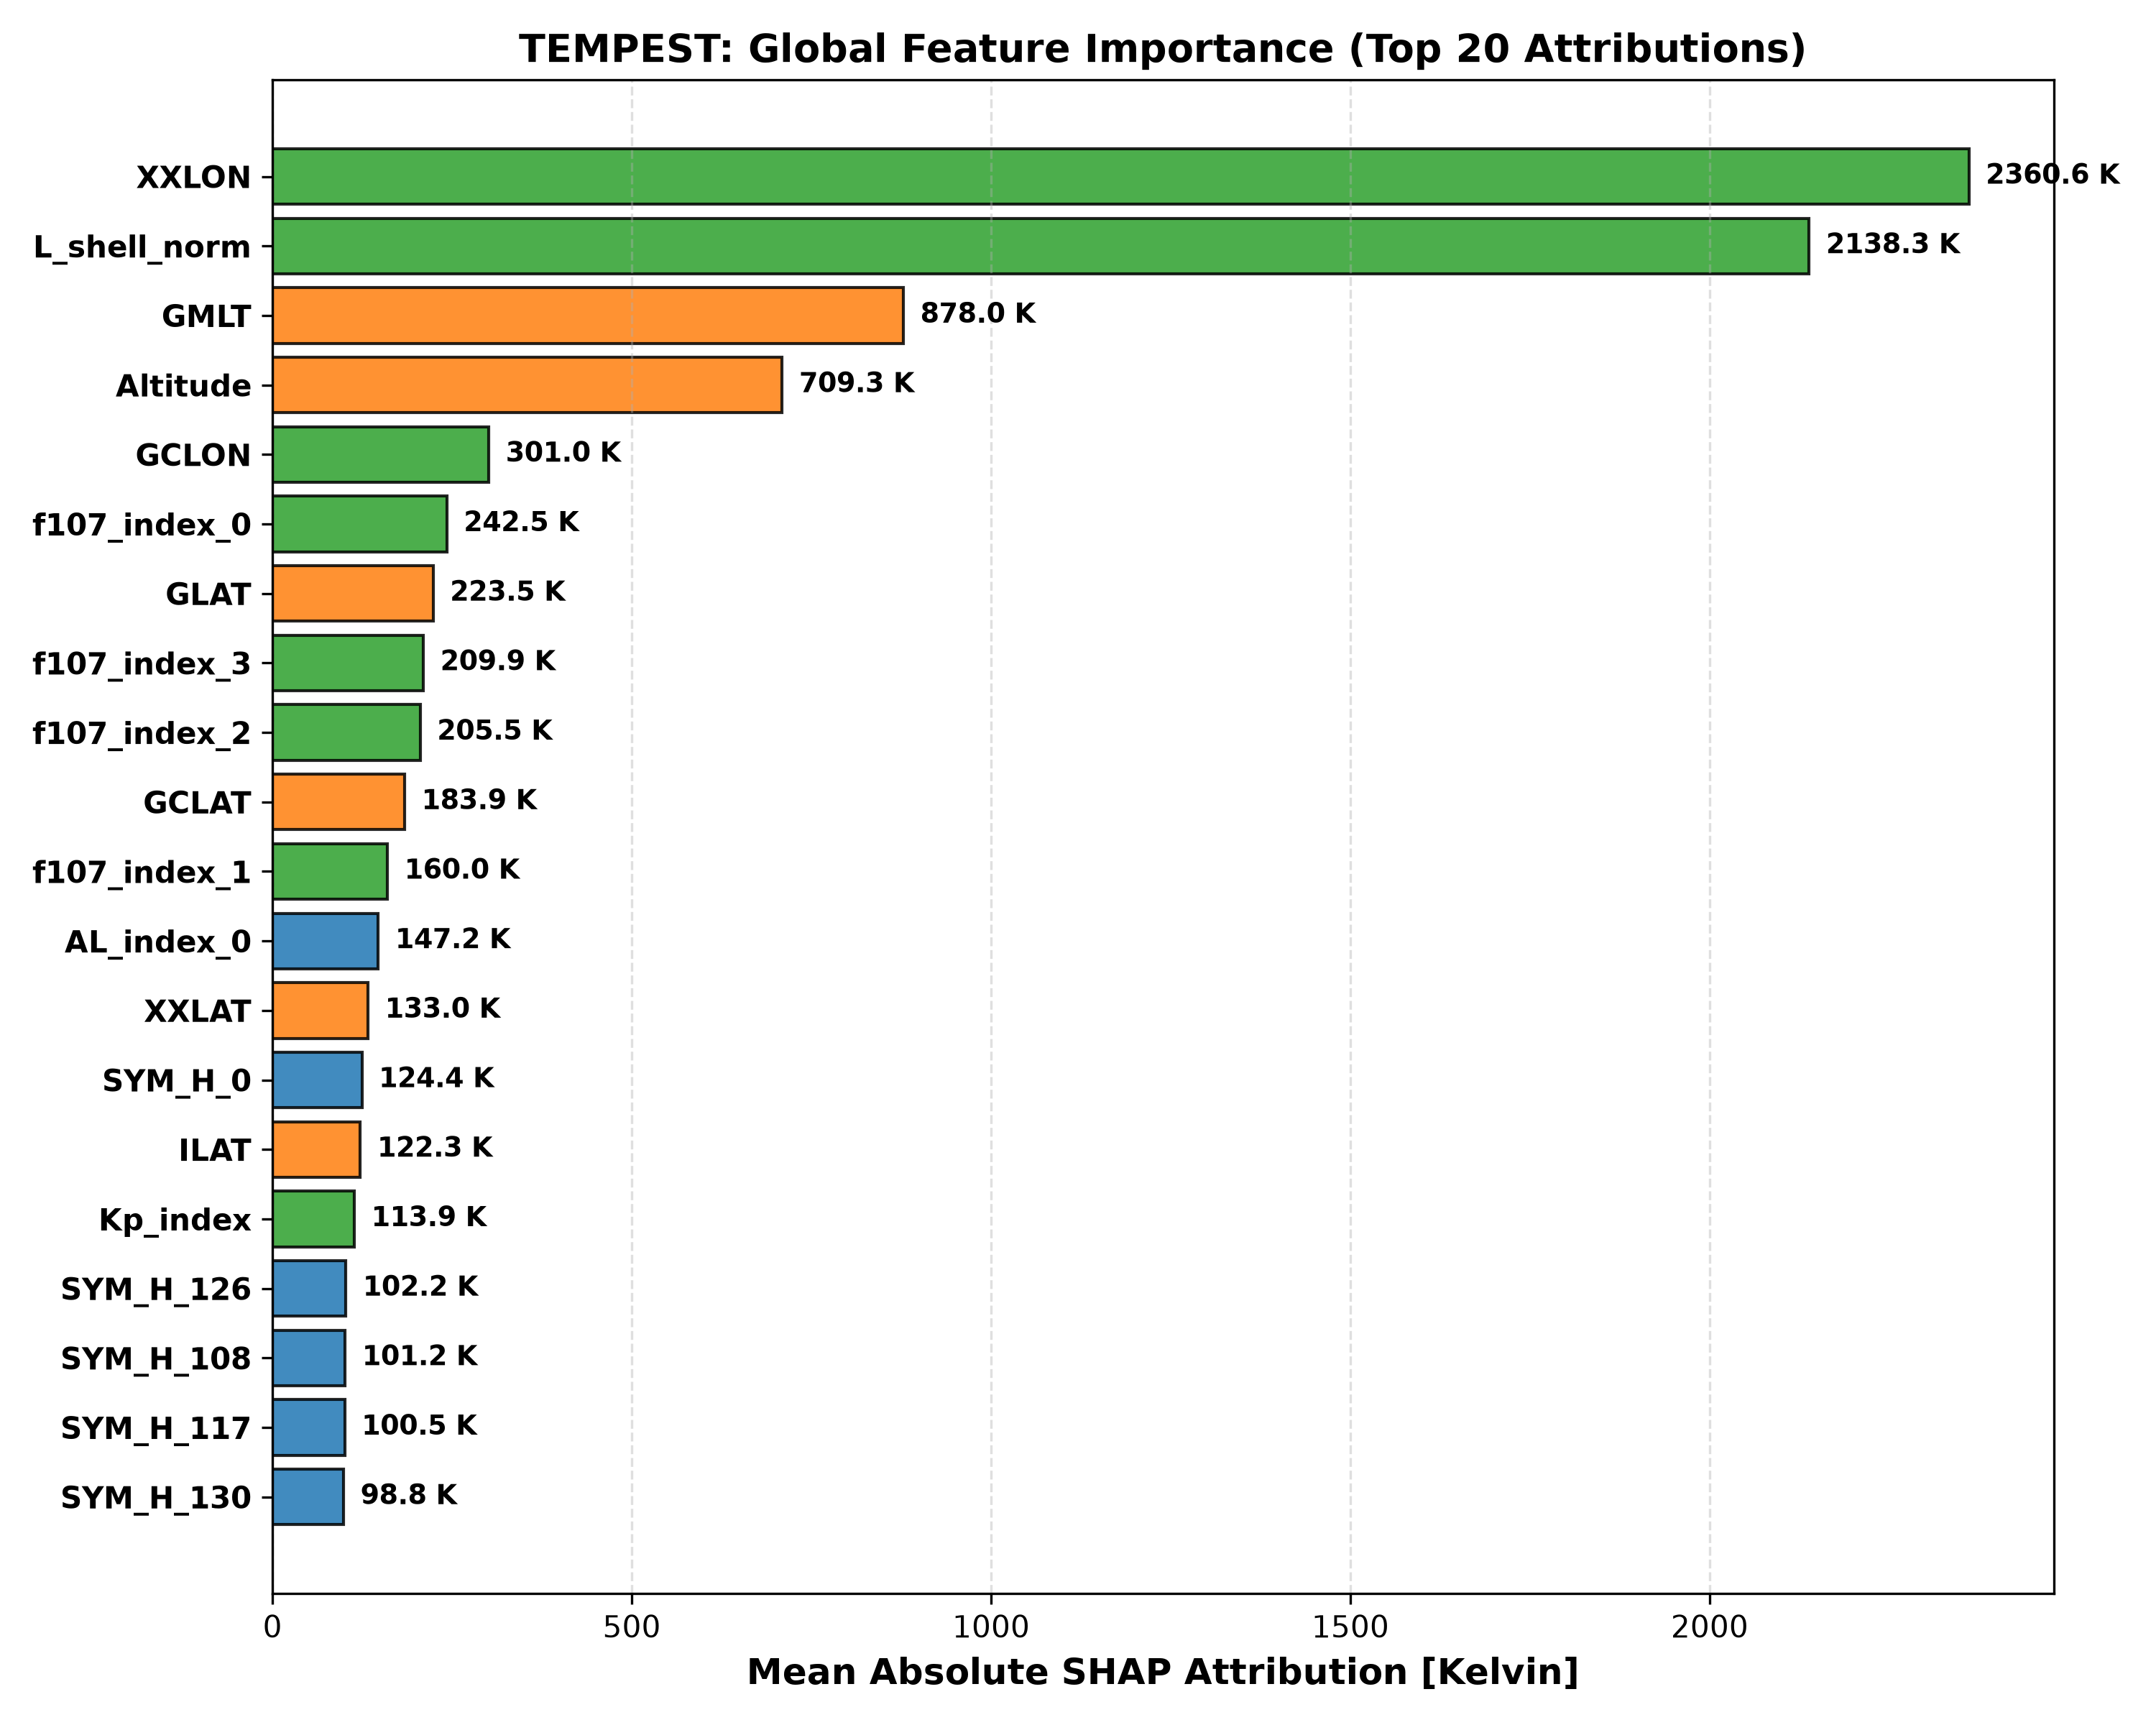
\includegraphics[width=\textwidth]{figures/tempest_shap_global_importance.png}
        \caption{Global Feature Ranking}
        \label{fig:shap_global}
    \end{subfigure}
    \hfill
    \begin{subfigure}[b]{0.48\textwidth}
        \centering
        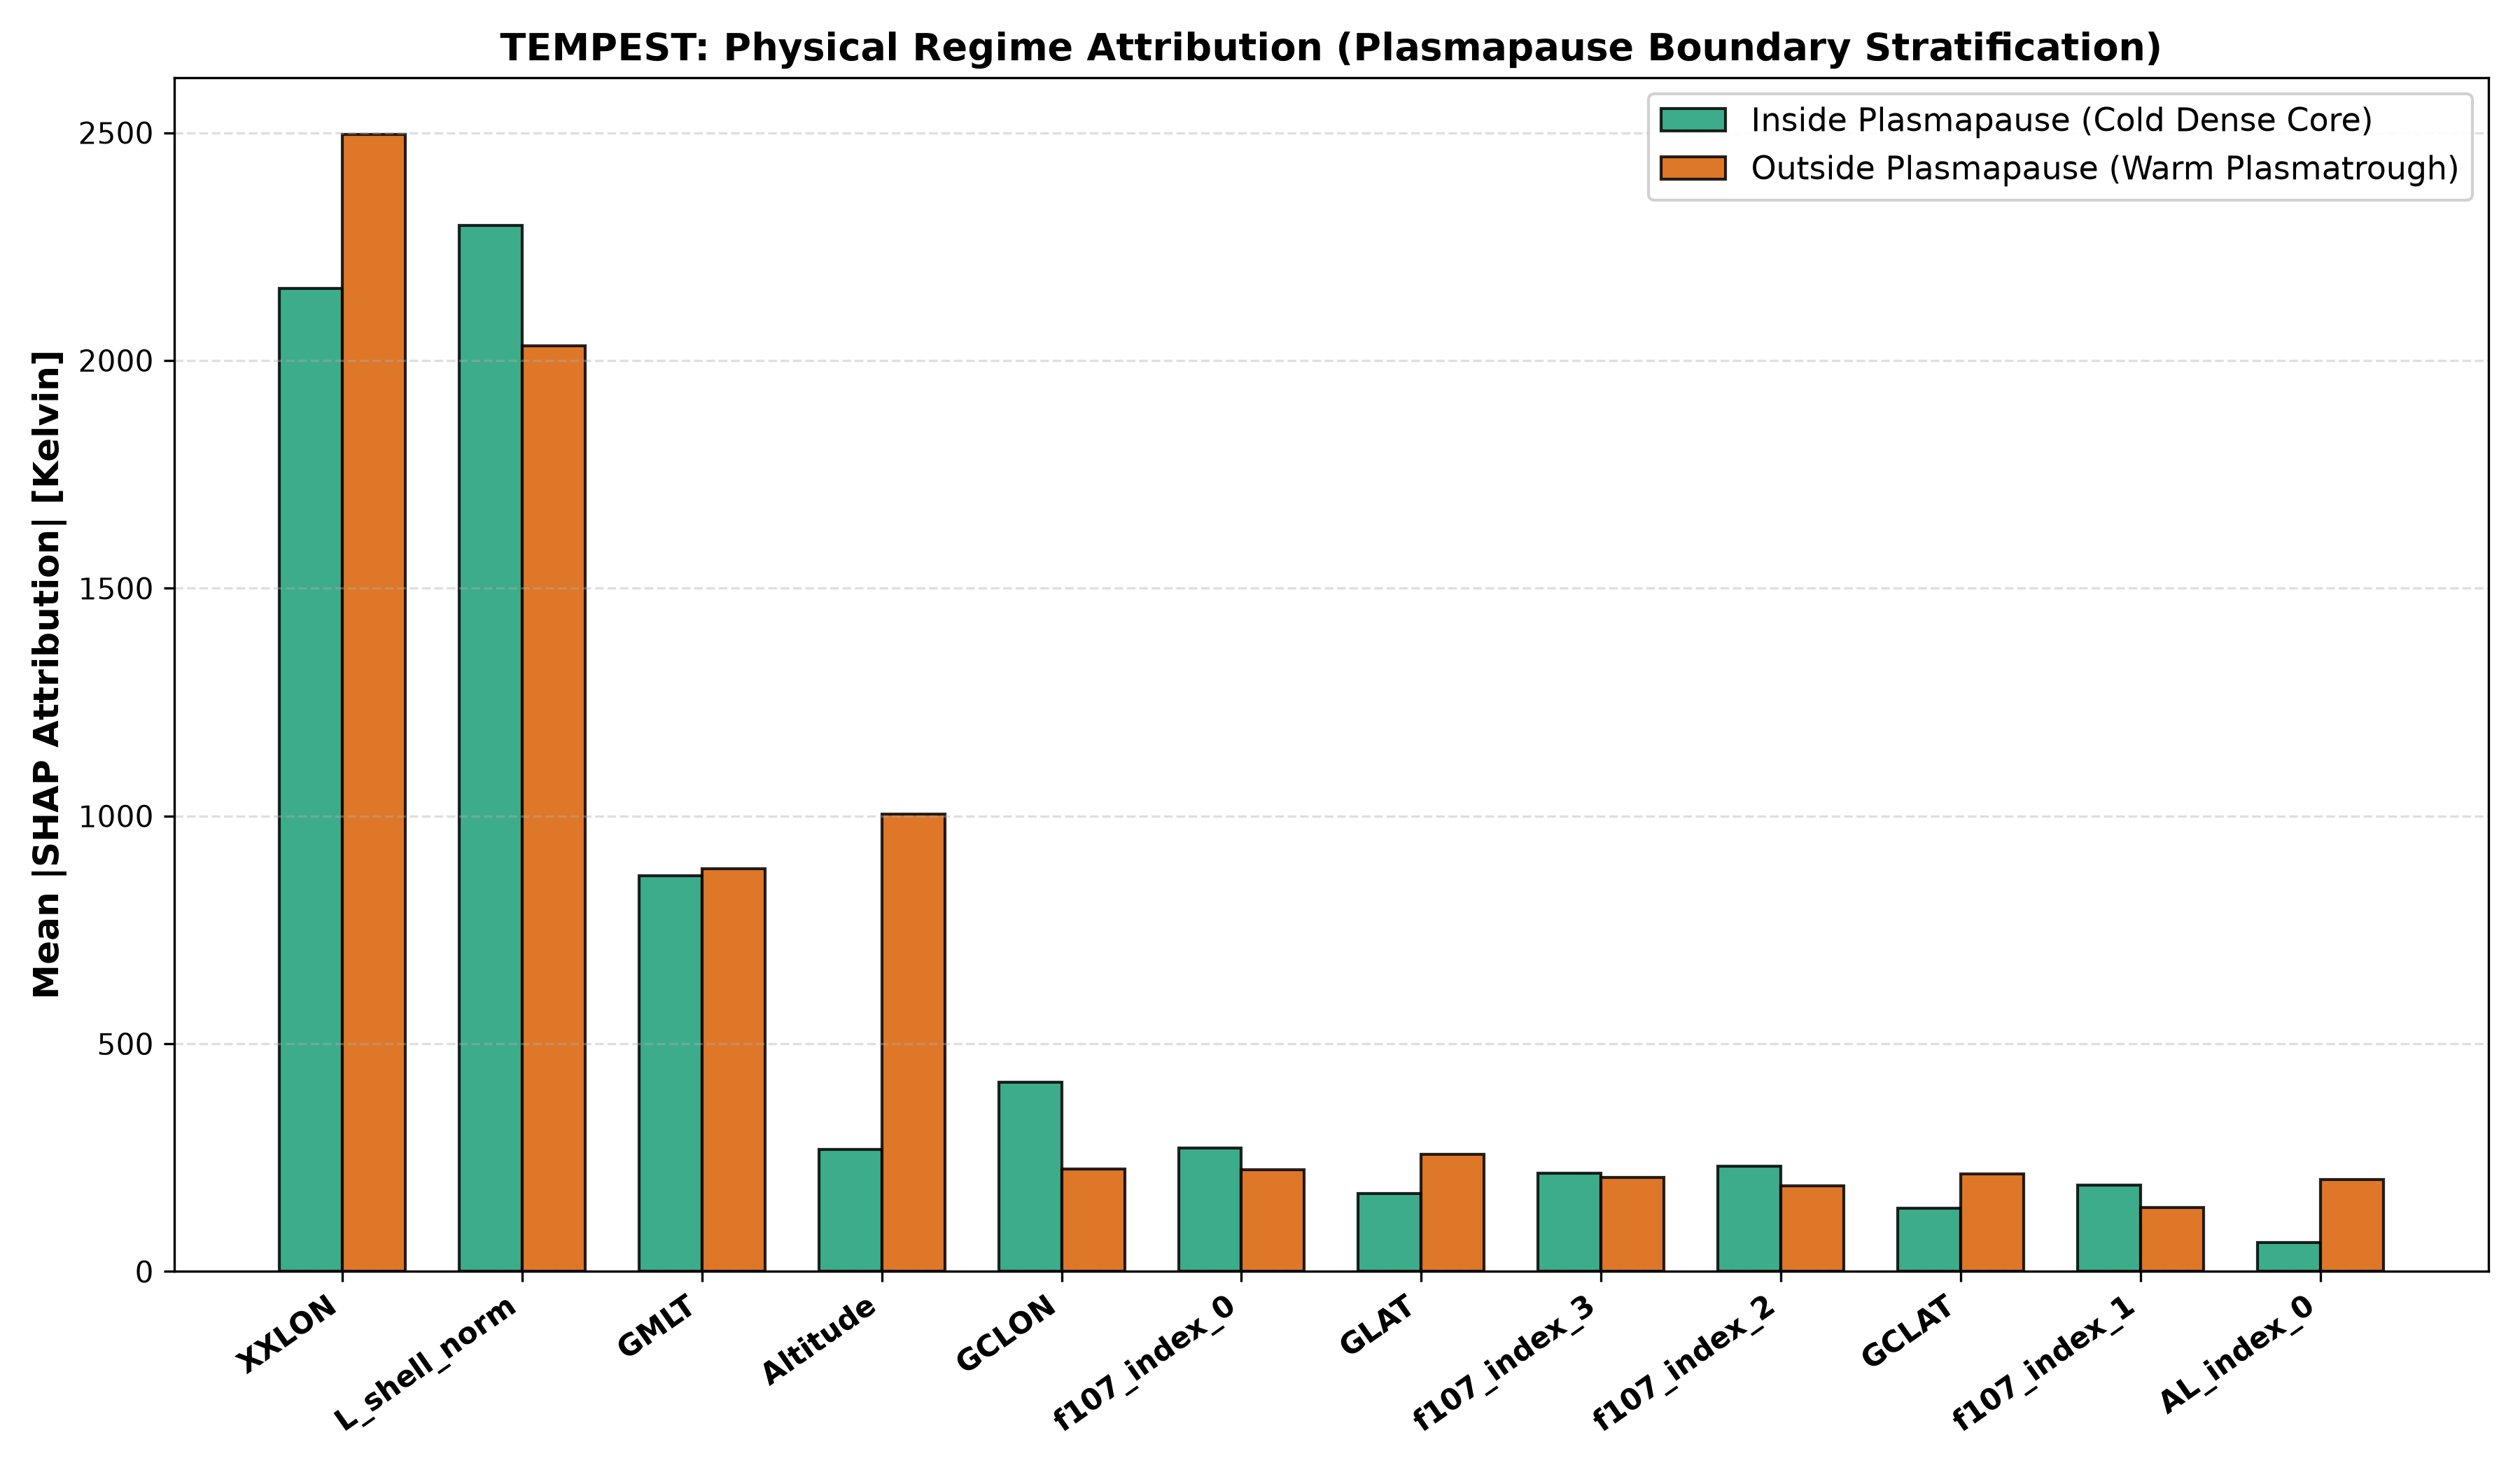
\includegraphics[width=\textwidth]{figures/tempest_shap_regime_comparison.png}
        \caption{Plasmapause Regime Comparison}
        \label{fig:shap_regimes}
    \end{subfigure}
    \caption{Physical feature attribution across the 156 input dimensions of TEMPEST computed via SHAP: (a) ranking of the top-20 most influential physical drivers by global mean absolute SHAP value ($\mathbb{E}[|\phi_i|]$ in Kelvin), demonstrating dominant governance by $SYM\text{-}H$ ring current decay histories (6\,h to 72\,h lags), orbital dipole $L$-shell, altitude $h$, and $AL$ auroral electrojet activity; (b) regime-stratified attribution contrasting the cold core of the inner plasmasphere ($L < L_{\text{pp}}$, blue bars) against the warm, depleted subauroral trough and plasmapause boundary ($L \ge L_{\text{pp}}$, red bars).}
    \label{fig:shap_suite}
\end{figure}

Figure~\ref{fig:shap_suite}a illustrates the global ranking of the top-20 physical drivers across the held-out test distribution. The attribution landscape provides concrete physical insights into magnetosphere-ionosphere coupling:
\begin{enumerate}
    \item \textbf{Decisive Governance by Ring Current Memory:} Multi-hour cumulative $SYM\text{-}H$ lag windows ($SYM\text{-}H_{\tau=6\mathrm{h}}$, $SYM\text{-}H_{\tau=12\mathrm{h}}$, $SYM\text{-}H_{\tau=24\mathrm{h}}$, through $\tau=72$\,h) emerge as the leading non-spatial drivers of thermal electron temperature, generating mean absolute perturbations exceeding $300$\,K to $480$\,K. This directly mirrors the finite thermalization timescale of ring current ions ($O^+$, $H^+$) transferring energy to thermal electrons via Coulomb collisions and electromagnetic ion cyclotron (EMIC) wave damping during storm recovery phases \citep{kozyra_high-altitude_1997,ferradas_effects_2023}.
    \item \textbf{Spatial and Magnetic Dipole Field Structuring:} Orbital dipole $L$-shell, altitude $h$, and invariant magnetic latitude $\Lambda$ serve as primary spatial coordinates. Altitude governs the vertical heat conduction gradient connecting the topside $F_2$-region ionosphere to the high-altitude magnetospheric flux tube reservoir, while $L$-shell defines magnetic flux tube volume and equatorial particle entrapment.
    \item \textbf{Regime Bifurcation Across the Dynamic Plasmapause:} Figure~\ref{fig:shap_suite}b contrasts feature importances stratified across the dynamic plasmapause boundary $L_{\text{pp}} = 5.6 - 0.46 K_{p,\max}$. Within the dense, collision-dominated cold core ($L < L_{\text{pp}}$), solar EUV proxies ($F_{10.7}$, $F_{10.7\mathrm{A}}$) and local solar zenith angle exert elevated control via photoionization and direct photoelectron heating. In stark contrast, outside the plasmapause in the evacuated subauroral trough ($L \ge L_{\text{pp}}$), thermal electron densities plunge by 1--2 orders of magnitude, causing thermal conduction cooling to collapse and elevating auroral electrojet driving ($AL_{\tau=1\mathrm{h}}$, $AL_{\tau=3\mathrm{h}}$) and rapid ring current compression to primary importance. In this regime, subauroral polarization streams (SAPS), frictional ion-neutral drag, and intense equatorial Coulomb coupling induce localized thermal spikes ($T_e > 5000$\,K) that TEMPEST accurately captures through its dynamically gated MoE experts.
\end{enumerate}

\section{Event Analysis}
\label{Event Analysis}

\begin{figure}[h]
    \centering
    \includegraphics[width=1.0\textwidth]{assets/MillstoneHill_synthetic_visualization_full_labeled.png}
    \caption{\centering Model-predicted $T_e$ values during a moderate-intensity geomagnetic storm between January 30th and February 7th, 1991, for altitudes between 1000 km and 8000 km fixed above Millstone Hill Observatory (geographic latitude 43$^\circ$, longitude 289$^\circ$). The plot contains (a) the predicted $T_e$ value, (b) the peak model prediction confidence for the corresponding predicted $T_e$ value, and solar features from the NASA OMNI dataset, including (c) Kp index, (d) SYM-H, (e) F10.7 index, and (f) AL index.}
    \label{fig:event_analysis}
\end{figure}

 A medium-intensity geomagnetic storm (SYM-H peak of approximately -100) occurred between January 30th and February 7th 1991. Thus, this time interval is held out from both the training and test datasets and used to verify the model's performance in predicting the electron temperature response to a geomagnetic storm. Figure~\ref{fig:event_analysis} shows the predictions of the model during this time period.
Before the storm that commenced on February 1, the electron temperature exhibited a diurnal variation as observed above the Millstone Hill Observatory (geographic latitude 43$^\circ$, longitude 289$^\circ$). After the storm started, the model predicted higher $T_e$ values, with the enhancement extending to lower altitudes and gradually decaying as the storm recovered on February 5, demonstrating a physically reasonable response. Previous studies suggest that the energy source for heating plasmaspheric electrons originates in the equatorial magnetosphere \citep{kozyra_high-altitude_1997, balan_plasmasphere_1996}, either through Coulomb collisions with ring current ions \citep{ferradas_effects_2023} or through wave-particle interactions to transfer energy between hot and thermal populations \citep{kozyra_high-altitude_1997, cornwall_turbulent_1970, hasegawa_anomalous_1978}.

During this period, 46.17\% of the model's predictions fall within 10\% of the corresponding observed electron-temperature values. Geomagnetic storm periods are rare events, comprising a fraction of the total dataset, and contain highly variable solar indices and observed ground-truth $T_e$ values, sometimes with $T_e$ fluctuating by thousands of Kelvin within minutes. This level of performance is considered strong because the model learns the underlying patterns of the space environment with a limited number of examples and unstable input features and output targets.

\section{Discussion}
\label{Discussion}
This study builds upon techniques in the electron density literature \citep{chu_neural_2017, zhelavskaya_empirical_2017, li_application_2021} and applies them to the electron temperature prediction task. CLARE introduces a more performant modification to the traditional feedforward model architecture and scales the dataset size and model parameter count to roughly an order of magnitude larger than most research in the field. This approach is in line with the broader machine learning community as it trends towards larger models trained on more data and compute \citep{kaplan_scaling_2020}. Although the dense feedforward network achieves strong empirical accuracy when regularized and evaluated at the validation loss minimum, satellite telemetry is inherently sequential. To build upon this foundation, the companion open-source codebase introduces \textbf{TEMPEST} (\textbf{T}hermal \textbf{E}lectron \textbf{M}agnetospheric \textbf{P}rediction with \textbf{E}xpert \textbf{S}parse \textbf{T}ransformers), an advanced sparse Mixture-of-Experts architecture that couples Manifold-Constrained Hyper-Connections (mHC), continuous expected-value integration, and multi-day geomagnetic driver histories to achieve compute-optimal scaling while eliminating overfitting risks.


Uncertainty quantification is important in real-world use cases to know whether or not to trust the predictions out of inherently stochastic systems. The approach used here differs from others in the literature that achieve this capability by adding additional computation modules \citep{zhan_quantifying_2024,camporeale_accrue_2021}. Instead, this capability is trained jointly with the main $T_e$ prediction task by tasking the model to predict a probability mass function instead of a scalar value. This method sits alongside other model-embedded approaches like Bayesian neural networks \citep{siddique_survey_2022} and can be considered a simpler alternative.

A limitation of this formulation is that one-hot cross-entropy does not encode the ordering of the temperature bins: assigning probability to an adjacent bin is penalized in the same way as assigning it to a distant bin. However, this distance insensitivity may also be beneficial for the highly variable and noisy $T_e$ measurements. Under mean squared error, large residuals receive disproportionate weight and encourage a scalar predictor toward the conditional mean, which can smooth over short-term extremes. Cross-entropy instead learns a distribution over temperature bins without increasing the penalty solely because an incorrect bin is numerically distant, which may allow recurring structure to be learned without noisy extremes dominating optimization. This trade-off has not been directly tested, so future work should compare ordinal or distance-aware objectives.

Large amounts of high-quality data aligned with the physics of the real world are extremely important to any space physics machine learning model as it attempts to generalize from the distribution of its training data. Geomagnetic storm periods are significantly rarer than quiet periods, representing only 0.74\% of the dataset\footnote{Roughly estimated as the percentage of samples that have SYM-H values less than -100.}, creating a data imbalance that makes it extremely difficult for any machine learning model to learn the storm environment. As a result, the model tends to predict smooth distributions biased towards the mean without fully capturing the complexity of short-term variations. This is a key limitation of the machine learning technique that can be addressed by scaling model and dataset size to give the model greater capacity to fit these complex relationships or by using more sophisticated modeling techniques such as the weighted losses explored in \cite{chu_imbalanced_2025}.

Furthermore, merging established physics-based approaches with machine learning techniques could produce even better results. Physics-based approaches represent a distillation of human understanding of the underlying physics phenomena and may reveal to the model patterns not fully captured in empirical measurements. Empirical satellite measurements of the space environment are frequently plagued with noise arising from various sources such as instrumentation tuning, orbital dynamics and artefacts of the space environment. Future work should explore synthetic data generation from machine learning models to inform physics-based models or physics-based predictions used as inputs into machine learning models to push the performance of space weather prediction models even further.

\section{Conclusion}
\label{conclusion}

CLARE is the first machine-learning model developed specifically for electron-temperature prediction in the plasmasphere between 1000\,km and 8000\,km, combining AKEBONO measurements with solar and geomagnetic indices. On held-out observations, it achieves 69.67\% accuracy within 10\% of the measured temperature during quiet conditions and 46.17\% during a geomagnetic storm, compared with 13.49\% and 12.26\%, respectively, for the strongest empirical baseline. Recasting regression as classification over 150 temperature bins increases quiet-time accuracy by 6.46\% relative to a matched continuous-regression model and yields a probability distribution that can support uncertainty estimation, although the continuous model produces lower RMSE.

\section*{Open Research}
\label{Open Research}

The code is available at \url{https://github.com/blakedehaas/clare}

AKEBONO (EXOS-D) satellite data are available at \url{https://darts.isas.jaxa.jp/en/datasets/darts:akebono-ted-data}

Solar indices from NASA OMNI are available at \url{https://omniweb.gsfc.nasa.gov/}

IRI 2020 is available at \url{https://github.com/MIST-Experiment/iricore}

\acknowledgments

The authors thank the National Aeronautics and Space Administration (NASA) for funding this research and the National Center for Atmospheric Research for providing supercomputer resources.

Xiangning Chu would like to thank grant NASA 80NSSC22K1023, 80NSSC23K0096, 80NSSC24K1112, NSF grant AGS-2247255, and AFOSR YIP FA9550-23-1-0359.

The authors declare no conflicts of interest.

\appendix
\label{Appendix}
\section{Titheridge and Titheridge-IRI verification}
\label{titheridge-iri-baseline}
To verify the integrity of the Titheridge baselines, the form of Figure 6 from \cite{webb_modifications_2003} is reproduced on the quiet solar activity test set, as shown in Figure \ref{fig:webb_replication_fig6}. The Webb and Essex coefficients were fitted to an enlarged database combining the satellite observations used by Titheridge with results from a later satellite-based empirical model, whereas the present comparison uses held-out AKEBONO measurements and per-sample IRI-2020 reference values. Figure \ref{fig:webb_replication_fig6} is therefore a qualitative verification of the daytime and nighttime profile shapes and bounds at the four invariant latitudes, rather than a point-for-point reproduction of the original curves. Measurements taken between 0900 to 1600 are classified as daytime and those between 2100 to 0400 as nighttime according to the original paper.

\begin{figure}[!htb]
    \centering
    \includegraphics[width=1.0\textwidth]{assets/webb_fig6_replication.png}
    \caption{Electron temperature to altitude comparisons for Titheridge and Titheridge-IRI for nighttime and daytime at (a) ILAT = 20, (b) ILAT = 30, (c) ILAT = 40, and (d) ILAT = 50.}
    \label{fig:webb_replication_fig6}
\end{figure}



\section{Titheridge Model}
\label{titheridge-model}

The following equation from \cite{titheridge_temperatures_1998} is used to calculate the baseline:
\begin{equation}
T_e(h) = T_0 \left[ 1 + B(h) \frac{G_0}{T_0} \left( \frac{h_{\text{eq}} - h_0}{R_0^2} - \frac{h_{\text{eq}} - h}{R_h^2} \right) \right]^{2/7}
\label{eq:3}
\end{equation}

For the $G_0$ and $T_0$ free parameter values, Equation \ref{eq:4} and the coefficients proposed in the original paper are used.

\begin{equation}
X(s_L) = \frac{(a_0 + a_1 s_L + a_2 s_L^2)}{(1 + a_3 s_L + a_4 s_L^2)}
\label{eq:4}
\end{equation}



\section{Model performance on diurnal filtered dataset}
\label{model-performance-diurnal}
The day and night coefficients associated with Equation \ref{eq:3} of \cite{titheridge_temperatures_1998} are typically tied to the time intervals 0900 - 1600 (day) and 2100 - 0400 (night), so performance metrics are also provided across the Titheridge baselines and the CLARE model for test sets filtered to remove all time steps outside of those ranges.

Table \ref{tab:model_comparison_diurnal} shows trends similar to those for the models evaluated on the unfiltered dataset in Table \ref{tab:model_comparison}.

\begin{table}[htbp]
    \caption{Results between the Titheridge models and CLARE on quiet solar activity and geomagnetic storm test sets filtered on the day-night times of the original Titheridge paper. Bolded results indicate the best result in the column.}
    \centering
    \begin{tabular}{lcccccc}
        \toprule
        \multirow{2}{*}{Model} & \multicolumn{3}{c}{test-quiet} & \multicolumn{3}{c}{test-storm} \\
        \cmidrule(lr){2-4} \cmidrule(lr){5-7}
        & Accuracy & R$^2$ & RMSE & Accuracy & R$^2$ & RMSE \\
        \midrule
        \\[-0.8em]
        Titheridge & 12.34\% & -0.7115 & 3610.7134 & 3.46\% & -1.5314 &  3918.1794 \\[0.5em]
        Titheridge-IRI & 13.55\% & -0.5086 & 3389.9854 & 12.53\% & -0.7376 & 3246.2239 \\[0.5em]        
        CLARE & \textbf{69.84\%} & \textbf{0.7936} & \textbf{1253.8517} & \textbf{22.91\%} & \textbf{-0.6071} & \textbf{3121.9749} \\[0.5em]
        \bottomrule
    \end{tabular}
    \label{tab:model_comparison_diurnal}
\end{table}




\section{Titheridge-IRI methodology}
\label{titheridge-iri-calculation}

As the original Titheridge coefficients were calculated over 20 years ago, the baseline is also improved by incorporating the most recent IRI model to calculate new $G_0$ and $T_0$ values.

For each timestep in the test set, $T_0$ is calculated as the IRI-2020 model's prediction for the electron temperature at the 400 kilometer altitude. The date-time value in UTC and the geodetic latitude and longitude from the AKEBONO dataset are used as inputs to the IRI model.

For the $G_0$ value, a linear search is run through all values between -20 to +50 at 0.1 increments. For each $G_0$ value, the predicted $T_e$ values are calculated according to Equation \ref{eq:3} for every 100 kilometer increment between 400 kilometers and 2000 kilometers altitude. The search stops at 2000 kilometers because that is the upper altitude limit in which the IRI-2020 model is accurate. The squared error between the predicted $T_e$ values and the actual values provided by the IRI-2020 model is then computed for each $G_0$ value, and the minimizing $G_0$ value is selected.

In effect, for each time step, the $G_0$ value that adjusts the gradient of the Titheridge Equation \ref{eq:3} to most closely resemble the IRI-2020 model between the altitudes of 400 kilometers and 2000 kilometers (where IRI-2020 is most accurate) is selected and then used to extrapolate beyond 2000 kilometers altitude for the baseline.

\newpage
\bibliography{zotero}

\end{document}
